% COMP2300 D2 - v3.8: authentic team-supplied annotated sketch sheets, dated receipt 19 November 2026, appendix with cross-references
\documentclass[12pt,a4paper]{article}

% -------------------------------------------------------------------------
% Page geometry and typography
% -------------------------------------------------------------------------
\usepackage[a4paper,margin=1.65cm,headheight=16pt,headsep=0.55cm,footskip=0.8cm]{geometry}
\usepackage[T1]{fontenc}
\usepackage[utf8]{inputenc}
\usepackage{lmodern}
\usepackage{microtype}
\usepackage{setspace}
\usepackage{parskip}

% -------------------------------------------------------------------------
% Tables, figures, diagrams and colour
% -------------------------------------------------------------------------
\usepackage{graphicx}
\usepackage{array,tabularx,booktabs,multirow,longtable}
\usepackage[table]{xcolor}
\usepackage{enumitem}
\usepackage{amsmath,amssymb}
\usepackage{tikz}
\usetikzlibrary{shapes.geometric,arrows.meta,positioning,calc,fit,backgrounds,decorations.pathreplacing}
\usepackage[most]{tcolorbox}
\usepackage{float}
\usepackage{caption}
\usepackage{titlesec}
\usepackage{tocloft}
\usepackage{fancyhdr}
\usepackage{lastpage}
\usepackage{hyperref}
\usepackage{bookmark}
\usepackage{placeins}
\usepackage{needspace}
\usepackage{xltabular}
% Float-only pages should never vertically centre screenshots leaving huge top gaps.
\makeatletter
\setlength{\@fptop}{0pt}
\setlength{\@fpsep}{12pt plus 2pt minus 2pt}
\setlength{\@fpbot}{0pt plus 1fil}
\makeatother
\renewcommand{\topfraction}{0.92}
\renewcommand{\textfraction}{0.08}
\renewcommand{\floatpagefraction}{0.60}
\setcounter{totalnumber}{6}
\setcounter{topnumber}{5}

% -------------------------------------------------------------------------
% Restrained academic palette
% -------------------------------------------------------------------------
\definecolor{Navy}{HTML}{17324D}
\definecolor{Teal}{HTML}{176B62}
\definecolor{TealPale}{HTML}{EEF5F3}
\definecolor{Slate}{HTML}{526477}
\definecolor{RuleGray}{HTML}{D8E0E6}
\definecolor{RowGray}{HTML}{F4F6F8}
\definecolor{Amber}{HTML}{A96512}
\definecolor{AmberPale}{HTML}{FBF5E9}
\definecolor{Alert}{HTML}{A33B3B}
\definecolor{AlertPale}{HTML}{FAEEEE}
\colorlet{brand}{Teal}
\colorlet{brandlight}{TealPale}
\colorlet{branddark}{Navy}
\colorlet{muted}{Slate}
\colorlet{accent}{Amber}
\colorlet{warningbg}{AmberPale}
\colorlet{alertred}{Alert}
\colorlet{RowAlt}{RowGray}

\hypersetup{
  colorlinks=true,
  linkcolor=Navy,
  urlcolor=Teal,
  citecolor=Navy,
  pdftitle={Footprint Lens: COMP2300 Deliverable 2 Conceptual Design Report},
  pdfauthor={Arnav Mishra, Keshav Singhal, Hiranya Makkar},
  bookmarksnumbered=true
}

% -------------------------------------------------------------------------
% Document rhythm and hierarchy
% -------------------------------------------------------------------------
\setlength{\parindent}{0pt}
\setlength{\parskip}{0.54em}
\setstretch{1.105}
\setlist[itemize]{leftmargin=1.45em,itemsep=0.34em,topsep=0.32em}
\setlist[enumerate]{leftmargin=1.7em,itemsep=0.36em,topsep=0.3em}
\setcounter{secnumdepth}{3}
\setcounter{tocdepth}{2}
% ---------------------------------------------------------------
% Editorial Table of Contents — 2 designed pages, auto-updating
% Section titles and page numbers still come from the .toc file.
% The typography, page chips, and links are not static artwork.
% ---------------------------------------------------------------
\makeatletter
\newlength{\tocrowsep}
\setlength{\tocrowsep}{0.29cm}

% Clear, compact navigation headers within the two-page contents spread.
\newcommand{\tocpagehead}[4]{%
  \noindent{\sffamily\footnotesize\bfseries\color{Teal}FOOTPRINT LENS}\hfill
  {\sffamily\footnotesize\bfseries\color{Slate}D2\ /\ CONTENTS \textcolor{Teal}{#1 / 02}}\par
  \vspace{0.38cm}
  {\sffamily\fontsize{29}{33}\selectfont\bfseries\color{Navy}Contents}\hfill
  {\sffamily\fontsize{17}{20}\selectfont\bfseries\color{Teal}#2}\par
  \vspace{0.16cm}
  {\color{Teal}\hrule height 1.0pt}\par
  \vspace{0.32cm}
  \noindent
  \begin{minipage}[c]{0.74\linewidth}
    {\sffamily\footnotesize\bfseries\color{Teal}\MakeUppercase{#3}}\par
    \vspace{0.1cm}
    {\sffamily\small\color{Slate}#4}\par
  \end{minipage}\hfill
  \begin{minipage}[c]{0.22\linewidth}
    \begin{tikzpicture}[x=1cm,y=1cm]
      \fill[TealPale] (0,0) rectangle (1.47,0.54);
      \ifnum#1=1
        \fill[Teal] (0,0) rectangle (0.74,0.54);
        \node[font=\sffamily\footnotesize\bfseries,text=white] at (0.37,0.27) {01};
        \node[font=\sffamily\footnotesize\bfseries,text=Slate] at (1.10,0.27) {02};
      \else
        \fill[Teal!16] (0,0) rectangle (0.74,0.54);
        \fill[Teal] (0.74,0) rectangle (1.47,0.54);
        \node[font=\sffamily\footnotesize\bfseries,text=Teal] at (0.37,0.27) {01};
        \node[font=\sffamily\footnotesize\bfseries,text=white] at (1.10,0.27) {02};
      \fi
    \end{tikzpicture}
  \end{minipage}\par
  \vspace{0.32cm}
}

% Section rows have a subtle tinted surface and their own compact folio.
\renewcommand*{\l@section}[2]{%
  \par\addvspace{0.52em}\noindent
  \begingroup
  \setlength{\fboxsep}{0pt}%
  \begin{tcolorbox}[enhanced,width=\linewidth,
       colback=RowGray!82,colframe=RowGray!82,
       boxrule=0pt,borderline west={2pt}{0pt}{Teal},
       arc=0.7mm,left=12pt,right=11pt,top=7pt,bottom=7pt,
       before skip=0pt,after skip=0pt]
   \noindent\begin{minipage}[t]{0.87\linewidth}
      \def\numberline##1{%
        \colorbox{TealPale}{\makebox[0.53cm][c]{\sffamily\small\bfseries\color{Teal}##1}}\hspace{0.26cm}}%
      {\sffamily\normalsize\bfseries\color{Navy}#1}%
   \end{minipage}\hfill
   \begin{minipage}[t]{0.085\linewidth}
     \raggedleft{\sffamily\normalsize\bfseries\color{Teal}#2}
   \end{minipage}
  \end{tcolorbox}
  \endgroup
  \par
}

% Subsection rows are quiet navigational details: no dot leaders.
\renewcommand*{\l@subsection}[2]{%
  \par\addvspace{0.12em}\noindent
  \hspace*{0.63cm}%
  \begin{minipage}[t]{0.79\linewidth}
    \begingroup
    \def\numberline##1{{\sffamily\footnotesize\bfseries\color{Teal}##1}\hspace{0.38cm}}%
    {\sffamily\small\color{Slate}#1}%
    \endgroup
  \end{minipage}\hfill
  \begin{minipage}[t]{0.09\linewidth}
    \raggedleft{\sffamily\small\color{Slate}#2}
  \end{minipage}\par
}

% The head of the native TOC is supplied by the editorial preface below.
\renewcommand{\contentsname}{}
\setlength{\cftbeforetoctitleskip}{-1.2cm}
\setlength{\cftaftertoctitleskip}{0pt}
\renewcommand{\cfttoctitlefont}{\relax}
\renewcommand{\cftaftertoctitle}{}

% Deliberate break: 1–5 on page one; 6–11 and Appendix on page two.
\newcommand{\tocpagecontinuation}{%
  \par\vfill
  \noindent\begin{tcolorbox}[
     enhanced,colback=TealPale!40,colframe=RuleGray,boxrule=0.5pt,
     borderline west={2.6pt}{0pt}{Teal},arc=1.2mm,
     left=12pt,right=12pt,top=10pt,bottom=10pt,
     before skip=0pt,after skip=0pt]
    {\sffamily\footnotesize\bfseries\color{Teal}MARKING GUIDE \textbar\ WHERE THE EVIDENCE SITS}\par\vspace{0.18cm}
    \noindent\begin{tabularx}{\linewidth}{@{}>{\raggedright\arraybackslash}p{0.30\linewidth} >{\raggedright\arraybackslash}X@{}}
     {\sffamily\small\bfseries\color{Navy}Design concepts} & {\small Sections 2--4: divergent ideas, three alternatives and justified selection; sketches in Appendix A.}\\[0.16cm]
     {\sffamily\small\bfseries\color{Navy}Small user stories} & {\small Section 5: persona-linked epics, MoSCoW priorities and acceptance checks.}\\[0.16cm]
     {\sffamily\small\bfseries\color{Navy}Low-fi prototype} & {\small Section 6: Figma states, exceptional paths, accessibility and feasibility.}\\
    \end{tabularx}
  \end{tcolorbox}
  \vspace{0.18cm}
  \clearpage
  \tocpagehead{02}{/ evidence}{Prototype \& evidence}{Interactive states, feasibility, evaluation and original design sketches.}
}
\makeatother
\titleformat{\section}
  {\Large\bfseries\sffamily\color{Navy}}
  {\thesection}{0.65em}{}
  [\vspace{0.35em}{\color{Teal}\titlerule[1.1pt]}]
\titleformat{\subsection}
  {\large\bfseries\sffamily\color{Teal}}
  {\thesubsection}{0.6em}{}
\titleformat{\subsubsection}
  {\normalsize\bfseries\sffamily\color{Navy}}
  {\thesubsubsection}{0.6em}{}
\titlespacing*{\section}{0pt}{1.5em}{0.7em}
\titlespacing*{\subsection}{0pt}{1.15em}{0.48em}
\titlespacing*{\subsubsection}{0pt}{0.8em}{0.25em}

\captionsetup{
  font=small,
  labelfont={bf,color=Navy},
  textfont={color=Slate},
  justification=centering,
  skip=6pt
}
\renewcommand{\arraystretch}{1.28}
\arrayrulecolor{RuleGray}\setlength{\tabcolsep}{4.5pt}

% -------------------------------------------------------------------------
% Running header and footer
% -------------------------------------------------------------------------
\pagestyle{fancy}
\fancyhf{}
\fancyhead[L]{\small\sffamily\color{Slate}COMP2300 \textbar\ Deliverable 2}
\fancyhead[R]{\small\sffamily\color{Slate}Footprint Lens}
\fancyfoot[L]{\small\sffamily\color{Slate}Conceptual Design Report}
\fancyfoot[R]{\small\sffamily\color{Slate}\thepage}
\renewcommand{\headrulewidth}{0.45pt}
\renewcommand{\footrulewidth}{0pt}
\fancypagestyle{plain}{
  \fancyhf{}
  \fancyhead[L]{\small\sffamily\color{Slate}COMP2300 \textbar\ Deliverable 2}
  \fancyhead[R]{\small\sffamily\color{Slate}Footprint Lens}
  \fancyfoot[L]{\small\sffamily\color{Slate}Conceptual Design Report}
  \fancyfoot[R]{\small\sffamily\color{Slate}\thepage}
  \renewcommand{\headrulewidth}{0.45pt}
}

% -------------------------------------------------------------------------
% Reusable components
% -------------------------------------------------------------------------
\newcommand{\code}[1]{\texttt{#1}}
\providecommand{\rupee}{\text{INR~}}

\newtcolorbox{storybox}[2]{
  enhanced,breakable,
  colback=TealPale!17,
  colframe=Teal!44!white,
  colbacktitle=Navy,
  coltitle=white,
  fonttitle=\bfseries\sffamily,
  title={#1},
  boxrule=0.55pt,
  arc=1.5mm,
  left=10pt,right=10pt,top=8pt,bottom=8pt,
  before skip=12pt,after skip=12pt
}

\newtcolorbox{keybox}[1][]{
  enhanced,
  colback=RowGray,
  colframe=RuleGray,
  boxrule=0.55pt,
  arc=1.5mm,
  left=9pt,right=9pt,top=7pt,bottom=7pt,
  #1
}

% Academic marginal callouts: use only for key decisions or evidence boundaries.
\newtcolorbox{insightbox}[1]{
  enhanced,breakable,
  colback=TealPale!70,colframe=Teal!45!white,
  boxrule=0.35pt,borderline west={2.8pt}{0pt}{Teal},
  sharp corners,leftrule=0pt,
  left=12pt,right=12pt,top=9pt,bottom=9pt,
  fonttitle=\bfseries\sffamily\color{Navy},
  title={#1},colbacktitle=TealPale!70,coltitle=Navy,
  before skip=12pt,after skip=12pt
}
\newtcolorbox{cautionbox}[1]{
  enhanced,breakable,
  colback=AmberPale!60,colframe=Amber!35!white,
  boxrule=0.35pt,borderline west={2.8pt}{0pt}{Amber},
  sharp corners,leftrule=0pt,
  left=12pt,right=12pt,top=9pt,bottom=9pt,
  fonttitle=\bfseries\sffamily\color{Navy},
  title={#1},colbacktitle=AmberPale!60,coltitle=Navy,
  before skip=12pt,after skip=12pt
}
\newtcolorbox{jtbox}{
  enhanced,breakable,
  colback=TealPale!45,colframe=Teal!35!white,
  boxrule=0.5pt,arc=1mm,
  left=14pt,right=14pt,top=10pt,bottom=10pt,
  before skip=12pt,after skip=12pt
}


% Compact editorial motifs; restrained but visually discoverable.
\definecolor{Indigo}{HTML}{4D6487}
\definecolor{IndigoPale}{HTML}{F0F3F8}
\definecolor{Gold}{HTML}{B78230}
\newtcolorbox{chapterfocus}[1]{
  enhanced,breakable,colback=IndigoPale,colframe=Indigo!35!white,
  borderline west={3pt}{0pt}{Indigo},boxrule=0.45pt,
  arc=1.2mm,left=12pt,right=12pt,top=10pt,bottom=10pt,
  fonttitle=\bfseries\sffamily,coltitle=Navy,title={#1},
  before skip=10pt,after skip=13pt
}
\newtcolorbox{microstory}[2]{
  enhanced,breakable,colback=RowGray!78,colframe=RuleGray,
  borderline west={2.4pt}{0pt}{Teal},boxrule=0.4pt,
  arc=1mm,left=10pt,right=10pt,top=7pt,bottom=8pt,
  fonttitle=\bfseries\sffamily,coltitle=Navy,
  title={#1 \hfill {\footnotesize\normalfont #2}},
  before skip=6pt,after skip=7pt
}
\newcommand{\sectionlead}[2]{%
\begin{chapterfocus}{#1}#2\end{chapterfocus}}

% Image slots automatically render the named image when it is added to the
% Overleaf project. Until then, a clean, dimensioned placeholder is shown.
\newcommand{\imagepanel}[4]{%
  \begin{minipage}[t]{#1}
    \centering
    \IfFileExists{#2}{%
      \includegraphics[width=\linewidth,height=#3,keepaspectratio]{#2}%
    }{%
      \setlength{\fboxsep}{0pt}%
      \fcolorbox{RuleGray}{RowGray}{%
        \parbox[c][#3][c]{\dimexpr\linewidth-2\fboxrule\relax}{%
          \centering
          \parbox[c]{0.88\linewidth}{\centering\small\sffamily\bfseries\color{Navy}#4}\\[0.55em]
          {\small\sffamily\color{Slate}Image placeholder}\\[0.25em]
          {\footnotesize\sffamily\color{Slate}Add \code{#2} to the project folder to populate this space.}
        }%
      }%
    }%
  \end{minipage}%
}

% Linked screen evidence: screenshots supplied by the team on 18 November 2026.
% Cropped to the Figma frame boundary only.  No UI content has been redrawn.
% The blue/teal report styling is separate from the fixed-state wireframe.
\newcommand{\figmashot}[3]{%
  \begin{minipage}[t]{0.481\textwidth}\centering
    {\footnotesize\sffamily\bfseries\color{Navy}#1}\par\vspace{0.11cm}
    \href{https://www.figma.com/design/L1kEH28shvU8494m2Y7EnT?node-id=#2}{%
      \includegraphics[width=\linewidth,keepaspectratio]{evidence/figma/#3.png}}\par
  \end{minipage}%
}
\newcommand{\figmarow}[6]{%
  \figmashot{#1}{#2}{#3}\hfill\figmashot{#4}{#5}{#6}\par\vspace{0.28cm}%
}

% Flowchart styles
\tikzset{
  flowbox/.style={rectangle,rounded corners=2pt,draw=Teal,fill=TealPale,minimum width=2.6cm,minimum height=0.9cm,text centered,text width=2.5cm,font=\footnotesize\bfseries},
  flowproc/.style={rectangle,rounded corners=2pt,draw=Slate!75,fill=white,minimum width=2.5cm,minimum height=0.8cm,text centered,text width=2.4cm,font=\scriptsize},
  flowdec/.style={diamond,aspect=1.8,draw=Amber,fill=AmberPale,minimum width=2.2cm,minimum height=0.8cm,text centered,text width=1.9cm,font=\scriptsize\bfseries},
  flowalert/.style={rectangle,rounded corners=2pt,draw=Alert,fill=AlertPale,minimum width=2.5cm,minimum height=0.8cm,text centered,text width=2.4cm,font=\scriptsize\bfseries},
  flowterminal/.style={rectangle,rounded corners=2pt,draw=Navy,fill=Navy,text=white,minimum width=2.4cm,minimum height=0.8cm,text centered,text width=2.3cm,font=\scriptsize\bfseries},
  flowarrow/.style={thick,-{Stealth[length=2mm]},draw=Teal},
  backarrow/.style={thick,dashed,-{Stealth[length=2mm]},draw=Slate},
  alertarrow/.style={thick,-{Stealth[length=2mm]},draw=Alert}
}

\begin{document}

% -------------------------------------------------------------------------
% Cover page
% -------------------------------------------------------------------------
% -------------------------------------------------------------------------
% Redesigned Footprint Lens cover page (D2)
% -------------------------------------------------------------------------
\begin{titlepage}
\thispagestyle{empty}
\setlength{\parskip}{0pt}
\vspace*{0.25cm}

% Institution identity
\noindent
\begin{minipage}[c]{0.69\textwidth}
  
\includegraphics[width=6.4cm,keepaspectratio]{southampton-delhi-logo-cropped.png}
\end{minipage}%
\begin{minipage}[c]{0.31\textwidth}
  \raggedleft
  {\sffamily\footnotesize\bfseries\color{Navy}COMP2300}\\[0.12cm]
  {\sffamily\scriptsize\color{Slate}DELIVERABLE 02}
\end{minipage}\par
\vspace{0.22cm}
{\color{RuleGray}\hrule height 0.9pt}

\vspace{0.78cm}
{\sffamily\footnotesize\bfseries\color{Teal} SOFTWARE DESIGN AND DEVELOPMENT PROJECT\par}
\vspace{0.17cm}
{\sffamily\bfseries\color{Navy}\fontsize{34}{40}\selectfont Footprint Lens\par}
\vspace{0.10cm}
{\sffamily\bfseries\color{Teal}\fontsize{17}{22}\selectfont Contextual Choice Coach\par}
\vspace{0.50cm}
{\sffamily\color{Slate}\fontsize{14}{19}\selectfont Deliverable 2: Conceptual Design Report\par}
\vspace{0.16cm}
{\sffamily\color{Slate}\small India-centric carbon footprint awareness and actionable reduction\par}

\vspace{0.62cm}
{\color{Teal}\rule{1.30cm}{2pt}}\par
\vspace{0.25cm}
{\sffamily\footnotesize\bfseries\color{Teal}
RESEARCH-LED CONCEPTS\hspace{0.65em}/\hspace{0.65em}
TESTABLE STORIES\hspace{0.65em}/\hspace{0.65em}
CLICKABLE LOW-FI DESIGN\par}

\vspace{0.68cm}
\begin{tcolorbox}[
  colback=RowGray,colframe=RuleGray,boxrule=0.55pt,
  borderline west={2.5pt}{0pt}{Teal},
  arc=1.5mm,left=11pt,right=11pt,top=9pt,bottom=9pt,
  before skip=0pt,after skip=0pt
]
  {\sffamily\bfseries\color{Navy}Design focus\par}
  \vspace{0.16cm}
  {\small A low-friction concept that makes everyday environmental
  estimates understandable, exposes their assumptions, respects non-negotiable
  constraints, and protects the boundary between shared and personal household data.\par}
\end{tcolorbox}

\vspace{0.70cm}
% Team contacts and academic supervision
\noindent
\begin{minipage}[t]{0.617\textwidth}
\begin{tcolorbox}[
  colback=white,colframe=RuleGray,boxrule=0.6pt,
  arc=1.4mm,height=3.55cm,valign=top,
  left=9pt,right=8pt,top=9pt,bottom=6pt,
  before skip=0pt,after skip=0pt
]
  {\sffamily\small\bfseries\color{Teal}PROJECT TEAM\par}
  \vspace{0.18cm}
  {\color{RuleGray}\hrule height 0.6pt}
  \vspace{0.17cm}
  \begingroup
  \setlength{\parskip}{0pt}
  \noindent{\sffamily\small\bfseries\color{Navy}Arnav Mishra}\hfill{\sffamily\footnotesize\href{mailto:am31g25@soton.ac.uk}{am31g25@soton.ac.uk}}\par
  \vspace{0.25cm}
  \noindent{\sffamily\small\bfseries\color{Navy}Keshav Singhal}\hfill{\sffamily\footnotesize\href{mailto:ks3e25@soton.ac.uk}{ks3e25@soton.ac.uk}}\par
  \vspace{0.25cm}
  \noindent{\sffamily\small\bfseries\color{Navy}Hiranya Makkar}\hfill{\sffamily\footnotesize\href{mailto:hm8g25@soton.ac.uk}{hm8g25@soton.ac.uk}}\par
  \endgroup
\end{tcolorbox}
\end{minipage}\hfill
\begin{minipage}[t]{0.355\textwidth}
\begin{tcolorbox}[
  colback=TealPale!47,colframe=RuleGray,boxrule=0.6pt,
  arc=1.4mm,height=3.55cm,valign=top,
  left=10pt,right=8pt,top=9pt,bottom=6pt,
  before skip=0pt,after skip=0pt
]
  {\sffamily\small\bfseries\color{Teal}PROJECT SUPERVISOR\par}
  \vspace{0.18cm}
  {\color{RuleGray}\hrule height 0.6pt}
  \vspace{0.22cm}
  {\sffamily\small\bfseries\color{Navy}Dr Pramod Gaur\par}
  \vspace{0.16cm}
  {\sffamily\footnotesize\href{mailto:P.Gaur@soton.ac.uk}{P.Gaur@soton.ac.uk}\par}
  \vspace{0.36cm}
  {\sffamily\scriptsize\color{Slate}Academic supervision\par}
\end{tcolorbox}
\end{minipage}\par

\vspace{0.55cm}
% Report details
{\sffamily\small\bfseries\color{Teal}REPORT DETAILS\par}
\vspace{0.18cm}
{\color{RuleGray}\hrule height 0.6pt}
\vspace{0.15cm}
{\small
\renewcommand{\arraystretch}{1.13}
\begin{tabularx}{\textwidth}{@{}>{\sffamily\bfseries\color{Navy}}l@{\hspace{0.85cm}}X@{}}
Module & COMP2300 Software Design and Development Project\\
Authors & Arnav Mishra \textbar\ Keshav Singhal \\
Department & Electronics and Computer Science, University of Southampton\\
%%Version & Version 3.9 : final editorial and pagination refinement\\
Date & November 20\textsuperscript{th}, 2026\\
\end{tabularx}
}

%\vspace{0.48cm}
%\noindent
%{\sffamily\footnotesize\bfseries\color{Teal}INTERACTIVE LOW-FIDELITY PROTOTYPE}\hfill
%\href{https://www.figma.com/design/L1kEH28shvU8494m2Y7EnT}{\sffamily\footnotesize\underline{Open Footprint Lens in Figma}}\par
%\vspace{0.19cm}
%{\color{RuleGray}\hrule height 0.9pt}
%\vspace{0.17cm}
%{\sffamily\footnotesize\color{Slate}Prepared as a design specification and evidence-led progression from Deliverable 1.\par}
\end{titlepage}

% -------------------------------------------------------------------------
% Abstract and contents
% -------------------------------------------------------------------------
\pagenumbering{roman}
\section*{Abstract}
\addcontentsline{toc}{section}{Abstract}
Deliverable 2 translates the D1 research baseline into a conceptual design for \textbf{Footprint Lens}, an India-centric carbon-footprint awareness and reduction tool. Three distinct interaction paradigms are compared: the \emph{Contextual Choice Coach}, the \emph{Household Commons Board}, and the \emph{Quiet-Week Action Cards}. A weighted multi-criteria decision analysis selects Concept A for detailed design because it combines low-friction activity capture, inspectable assumptions, constraint-aware action handling and explicit shared-household boundaries. The report specifies a MoSCoW-prioritised user-story register, a linked Figma click-through illustrating the P0--P6 low-fidelity interaction model, a formative evaluation protocol, and the proposed technical direction. Annotated sketch evidence and its provenance limitations are provided in Appendix~\ref{app:ideation}. Design claims are distinguished from prototype behaviour and outcomes that still require user evaluation.

\vspace{0.44cm}
\noindent{\sffamily\footnotesize\bfseries\color{Teal}REPORT AT A GLANCE}\par
\vspace{0.22cm}
\noindent
\begin{minipage}[t]{0.315\textwidth}
\begin{tcolorbox}[height=4.72cm,enhanced,colback=RowGray,colframe=RuleGray,
  boxrule=0.55pt,arc=1.4mm,borderline north={2.5pt}{0pt}{Teal},
  left=10pt,right=9pt,top=11pt,bottom=8pt,before skip=0pt,after skip=0pt]
{\sffamily\color{Teal}\large\bfseries 01}\par\vspace{0.12cm}
{\sffamily\color{Navy}\small\bfseries Design exploration}\par\vspace{0.10cm}
{\sffamily\scriptsize\bfseries\color{Teal}Sections 1--4; Appendix A}\par\vspace{0.18cm}
{\small\raggedright D1 findings, three distinct concepts, selection rationale and annotated sketches.\par}
\end{tcolorbox}
\end{minipage}\hfill
\begin{minipage}[t]{0.315\textwidth}
\begin{tcolorbox}[height=4.72cm,enhanced,colback=TealPale!55,colframe=RuleGray,
  boxrule=0.55pt,arc=1.4mm,borderline north={2.5pt}{0pt}{Teal},
  left=10pt,right=9pt,top=11pt,bottom=8pt,before skip=0pt,after skip=0pt]
{\sffamily\color{Teal}\large\bfseries 02}\par\vspace{0.12cm}
{\sffamily\color{Navy}\small\bfseries Stories and prototype}\par\vspace{0.10cm}
{\sffamily\scriptsize\bfseries\color{Teal}Sections 5--6}\par\vspace{0.18cm}
{\small\raggedright Small user stories, testable criteria and the clickable P0--P6 Figma states.\par}
\end{tcolorbox}
\end{minipage}\hfill
\begin{minipage}[t]{0.315\textwidth}
\begin{tcolorbox}[height=4.72cm,enhanced,colback=RowGray,colframe=RuleGray,
  boxrule=0.55pt,arc=1.4mm,borderline north={2.5pt}{0pt}{Teal},
  left=10pt,right=9pt,top=11pt,bottom=8pt,before skip=0pt,after skip=0pt]
{\sffamily\color{Teal}\large\bfseries 03}\par\vspace{0.12cm}
{\sffamily\color{Navy}\small\bfseries Evaluation and evidence}\par\vspace{0.10cm}
{\sffamily\scriptsize\bfseries\color{Teal}Sections 7--11}\par\vspace{0.18cm}
{\small\raggedright Proposed user evaluation, team process and limits of the design evidence.\par}
\end{tcolorbox}
\end{minipage}\par
\vspace{0.35cm}
\begin{insightbox}{Evidence boundary}
The Figma prototype illustrates planned interaction through fixed states. Functional implementation and participant usability evaluation are future work, not results claimed in D2.
\end{insightbox}

%%% Table of Contents

\clearpage
\begingroup
\makeatletter
\setlength{\parskip}{0pt}
\setstretch{1}
\newcounter{tocsecn}\setcounter{tocsecn}{0}

% Shared geometry: section and subsection rows end on the same right edge
\def\tocfolio{1.2cm}   % page-number column width
\def\tocrin{11pt}      % right inset

% Header, shared by both pages
\newcommand{\tochead}[2]{%
  \noindent{\sffamily\bfseries\footnotesize\color{Teal}FOOTPRINT LENS}\hfill
  {\sffamily\bfseries\footnotesize\color{Slate}D2\ /\ CONTENTS\ \textcolor{Teal}{#1\,/\,2}}\par
  \vspace{6pt}
  \noindent{\sffamily\fontsize{28}{31}\selectfont\bfseries\color{Navy}Contents}\hfill
  {\sffamily\fontsize{15}{18}\selectfont\bfseries\color{Teal}#2}\par
  \vspace{3pt}
  {\color{Teal}\hrule height 1pt}\par
  \vspace{14pt}%
}

% Page break between the two halves (sections 1-6 | 7-Appendix)
\newcommand{\tocbreak}{%
  \par\vfill
  \noindent{\color{RuleGray}\rule{\linewidth}{0.6pt}}\par\vspace{5pt}
  {\sffamily\scriptsize\color{Slate}\textbf{\color{Teal}MARKING GUIDE}\enspace
  \textbf{Design concepts:} Sections 2--4 \enspace$\cdot$\enspace
  \textbf{Small user stories:} Section 5 \enspace$\cdot$\enspace
  \textbf{Low-fi prototype:} Section 6}\par
  \clearpage
  \tochead{2}{/ evidence}%
}

% Section rows
\renewcommand*{\l@section}[2]{%
  \stepcounter{tocsecn}%
  \ifnum\value{tocsecn}=8 \tocbreak\fi
  \par\addvspace{8pt}\noindent
  \begingroup
  \setlength{\fboxsep}{0pt}%
  \begin{tcolorbox}[enhanced,width=\linewidth,
       colback=RowGray!82,colframe=RowGray!82,
       boxrule=0pt,borderline west={2pt}{0pt}{Teal},
       arc=0.7mm,left=11pt,right=\tocrin,top=5pt,bottom=5pt,
       before skip=0pt,after skip=0pt]
   \noindent\begin{minipage}[t]{\dimexpr\linewidth-\tocfolio\relax}
      \def\numberline##1{%
        \colorbox{TealPale}{\makebox[0.52cm][c]{\sffamily\footnotesize\bfseries\color{Teal}##1}}\hspace{0.24cm}}%
      {\sffamily\small\bfseries\color{Navy}#1}%
   \end{minipage}%
   \begin{minipage}[t]{\tocfolio}
     \raggedleft{\sffamily\small\bfseries\color{Teal}#2}%
   \end{minipage}
  \end{tcolorbox}
  \endgroup
  \par\vspace{3pt}
}

% Subsection rows
\renewcommand*{\l@subsection}[2]{%
  \par\noindent
  \hspace*{0.65cm}%
  \begin{minipage}[t]{\dimexpr\linewidth-0.65cm-\tocrin-\tocfolio\relax}
    \begingroup
    \def\numberline##1{{\sffamily\bfseries\color{Teal}##1}\hspace{0.32cm}}%
    {\fontsize{10}{14.5}\selectfont\sffamily\color{Slate}#1}%
    \endgroup
  \end{minipage}%
  \begin{minipage}[t]{\tocfolio}
    \raggedleft{\fontsize{10}{14.5}\selectfont\sffamily\color{Slate}#2}%
  \end{minipage}\hspace*{\tocrin}\par
}

\tochead{1}{/ research}
\@starttoc{toc}

% Closing note on page two
\par\vfill
\noindent{\color{RuleGray}\rule{\linewidth}{0.6pt}}\par\vspace{5pt}
{\sffamily\scriptsize\color{Slate}\textbf{\color{Teal}PROTOTYPE ACCESS}\enspace
The title page links to the clickable Figma file; individual screen figures are linked directly to their frames.}\par
\endgroup

%%%%%%% Section 1
\clearpage
\pagenumbering{arabic}
\setcounter{page}{1}

\section{Introduction, Problem Framing and Design Principles}

\subsection{Context and Problem Statement}
The official COMP2300 Topic 1 specification requires an interactive system that helps users understand everyday lifestyle routines affecting their carbon footprint and evaluate feasible reduction choices across transport, home energy, food, waste, and water. D1 documented design tensions in illustrative coursework interviews and its personas: shared or unmetered bills, constrained housing, seasonal heat, and safety-critical travel for shift workers \cite{d1report}. The transcripts inform design hypotheses, not population-level claims about India. Published work also identifies variation in Indian household footprints \cite{lee2021}. 

Carbon tracking and action apps already exist, and their interfaces vary. A critical HCI concern is that narrowly persuasive sustainability interfaces may oversimplify situated practices; this is a design risk, not proof that all competing tools behave alike \cite{brynjarsdottir2012}. Grounded in our D1 thematic synthesis (semantic themes S1--S3 and latent themes L1--L3), our guiding Job to Be Done (JTBD) is:
\begin{jtbox}
\itshape
When I want to understand how my everyday routines and household habits affect the environment, I want to see which activities matter most in terms I can picture and which realistic alternatives are open to me, so that I can make changes that fit my budget, safety, rota, and shared home without being misled, lectured, or blamed for constraints I cannot control.
\end{jtbox}

\begin{chapterfocus}{What the selected experience must achieve}
\vspace{-0.9em}
\renewcommand{\arraystretch}{1}
\setlength{\parskip}{0pt}
\setlength{\tabcolsep}{0pt}
\begin{tabularx}{\linewidth}{@{}X@{\hspace{12pt}}X@{\hspace{12pt}}X@{}}
{\sffamily\bfseries\color{Teal}1\enspace}{\bfseries\color{Navy}Understand the number}\par\vspace{1pt}
{\small\color{Slate}Inspect the factor and source.}
&
{\sffamily\bfseries\color{Teal}2\enspace}{\bfseries\color{Navy}Respect the constraint}\par\vspace{1pt}
{\small\color{Slate}No guilt for necessary travel.}
&
{\sffamily\bfseries\color{Teal}3\enspace}{\bfseries\color{Navy}Protect shared data}\par\vspace{1pt}
{\small\color{Slate}No inferred flatmate share.}
\end{tabularx}
\vspace{-0.4em}
\end{chapterfocus}

\subsection{Core Design Principles}
To preserve rigorous traceability to our D1 empirical baseline, the system adheres to five fundamental design principles:
\begin{enumerate}[label=\textbf{\color{Teal}DP\arabic*.},leftmargin=*,itemsep=0.68em,topsep=0.5em]
  \item \textbf{Transparent Provenance (S1, E2):} Every numeric emission estimate must explicitly expose its formula, activity quantity, conversion factor, reference year, geographic applicability, and evidence boundary. Where no verified India-specific factor exists, the system must show an \emph{estimate unavailable} state rather than fabricating a number.
  \item \textbf{Constraint-Aware Protection (L3, E3):} Necessary routines driven by personal safety, night curfews, medical cooling, or tenancy rules must be flaggable as \emph{protected}, immediately disabling punitive advice or moralistic judgment.
  \item \textbf{Low-Burden, Two-Way Navigation (S3, E5):} Core estimation must require $\le 3$ primary decisions ($\le 60$ seconds). Users must be able to explore assumptions or backtrack without destructive state loss.
  \item \textbf{Communal Boundary Integrity (L1/L2, E7):} Shared utilities (e.g., central geysers, air conditioning, delivery packaging) must be displayed as collective household totals and never artificially partitioned into an individual's personal score without verified sub-metering.
  \item \textbf{Descriptive Representation for Circular Habits (S2, E4):} Indigenous Indian conservation practices (e.g., kabadiwala recycling, bucket baths, appliance repair) must be acknowledged descriptively without claiming unverified carbon offsets.
\end{enumerate}

\subsection{From Research Findings to Design Controls}
The principles above are not decorative statements: each creates a constraint on the interaction and on what the system is permitted to claim. Table~\ref{tab:design-controls} makes that translation explicit and provides a reviewable bridge from D1 themes to the P0--P6 design.

\begin{table}[ht]
\centering
\small
\caption{Traceability from D1 design drivers to interaction controls and verification}
\label{tab:design-controls}
\footnotesize
\setlength{\emergencystretch}{1em}
\begin{tabularx}{\textwidth}{@{}>{\raggedright\arraybackslash}p{2.7cm}>{\raggedright\arraybackslash}p{2.7cm}>{\raggedright\arraybackslash}X>{\raggedright\arraybackslash}p{2.7cm}@{}}
\toprule
\textbf{Driver} & \textbf{Control} & \textbf{Expected system behaviour} & \textbf{Verification}\\
\midrule
DP1: Transparent provenance & P2 result links to P3 assumptions & Show quantity, unit, factor, source status, geography, year where known, and formula; do not silently turn missing evidence into zero. & Inspect a known factor and an unavailable-factor case.\\
\rowcolor{brandlight}
DP2: Constraint-aware protection & Protected flag at P0; guard at P4 & Protected routines receive no substitution prompt or penalty. The flag changes the available interaction, not the estimated physical impact. & Confirm protected and unprotected paths differ as specified.\\
DP3: Low-burden, reversible entry & P0--P2 primary path; edit/back navigation & Category owns its unit; invalid input returns actionable feedback without erasing valid fields. & Test valid, blank, negative and out-of-range quantities.\\
\rowcolor{brandlight}
DP4: Communal boundary integrity & Explicit scope and P6 boundary view & A shared meter remains a communal total unless reliable sub-metering and consent justify attribution. & Explain-back: communal kWh is not an individual's footprint.\\
DP5: Descriptive circularity & P5 descriptive record & Repair, reuse and composting can be recorded without fabricated avoided-emissions credits. & Confirm no unsupported numeric deduction is produced.\\
\bottomrule
\end{tabularx}
\end{table}


\subsection{D2 assessment evidence map}
The report is organised around the principal D2 evidence areas. The table below is a navigation aid for the marker; it does not claim that an artefact has been independently assessed or that planned evaluation has already taken place.

\begin{table}[H]
\centering
\small
\caption{Mapping of D2 assessment areas to report evidence}
\label{tab:assessment-map}
\begin{tabularx}{\textwidth}{@{}>{\raggedright\arraybackslash}p{3.1cm}>{\raggedright\arraybackslash}p{2.6cm}X@{}}
\toprule
\textbf{Assessment area} & \textbf{Report location} & \textbf{Evidence presented}\\
\midrule
Design concepts and selection & Sections 2--4 & Eight synthesised response families, three team-supplied annotated sketch sheets (Appendix~\ref{app:ideation}), distinct concepts, concept flowcharts, weighted selection rationale and novelty comparison.\\
\rowcolor{RowGray}
Small user stories & Section 5 & Fourteen D1-linked parent stories plus implementation-sized child stories with individual outcomes, priority inheritance, evidence and observable acceptance criteria.\\
Low-fidelity prototype & Section 6 & P0--P6 interaction model, state walkthrough, linked Figma screen states, actual grouped Figma screenshots, accessibility requirements and scoped technical verification.\\
\rowcolor{RowGray}
Evaluation and project process & Sections 7--9 & Proposed formative tasks and metrics, three-week progression, work products, collaboration approach and product/process reflection.\\
Report presentation and references & Throughout & A4 layout, 12-point body text, structured headings, figure/table captions and cited sources.\\
\rowcolor{RowGray}
AI-use disclosure & Separate submission artefact & Submit the team's completed \code{genai.txt} separately and verify names, tool versions, purposes and human review.\\
\bottomrule
\end{tabularx}
\end{table}

\section{Ideation Process and Response Families}

The project materials identify eight response families, ranging from explain-and-compare journeys and household coordination to rota-aware action cards and offline conversation aids. Figure~\ref{fig:ideation_funnel} shows how these directions were synthesised into three distinguishable interaction models. A newly supplied annotated divergent-ideas sketch (Figure~\ref{fig:divergent_preview}; full sheet in Appendix~\ref{app:ideation}) illustrates seven prominent candidate directions and their initial keep/drop reasoning. It complements rather than replaces the broader eight-family synthesis.

\begin{cautionbox}{What the new sketches do and do not establish}
Three annotated sketch sheets were supplied for this revision on 19 November 2026 and are reproduced in Appendix~\ref{app:ideation}. They document the design alternatives, current selection argument and refinement questions. Their original session date, authorship details and whether they reproduce earlier notes still require team confirmation. Some sheets incorporate printed visual reference material. They are \emph{not} independent evidence of a dated historical brainstorming session, user testing or participant results. The eight-family map remains an analytic synthesis, not a raw idea-count record.
\end{cautionbox}

Concept A combines immediate feedback and inspectable assumptions; Concept B prioritises shared-home coordination; and Concept C prioritises periodic, constraint-filtered prompts. These are alternatives in user interaction, not three visual skins or three implemented products.

\begin{figure}[ht]
\centering
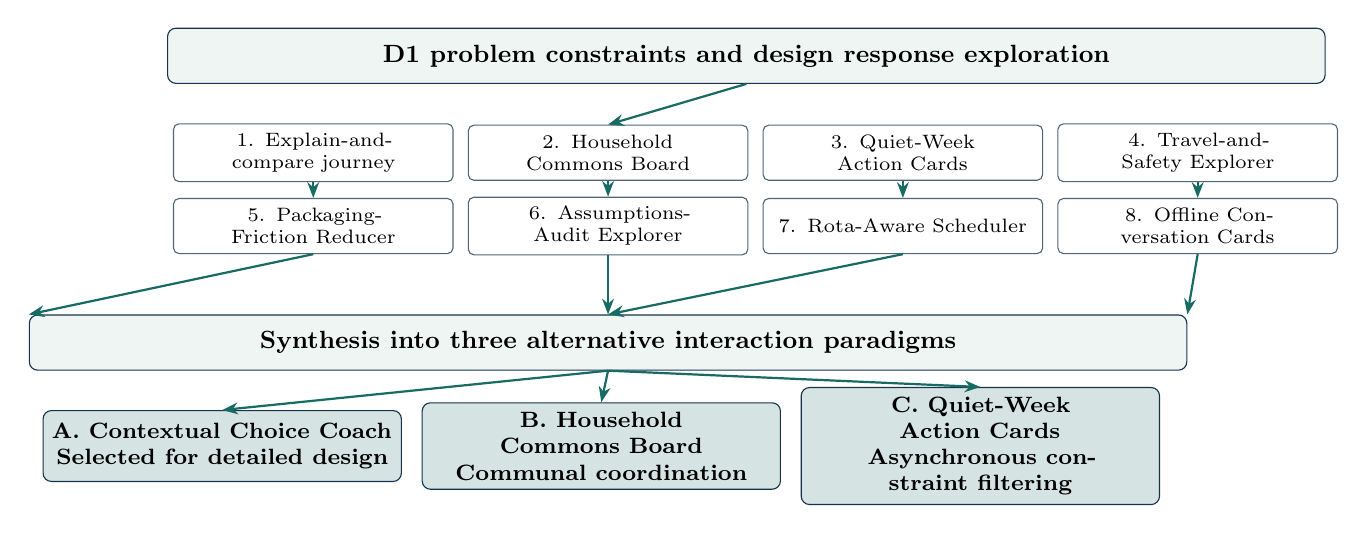
\begin{tikzpicture}[
  node distance=0.3cm and 0.2cm,
  stage/.style={rectangle,rounded corners=3pt,draw=branddark,fill=brandlight,minimum width=14.7cm,minimum height=0.7cm,text centered,font=\small\bfseries},
  family/.style={rectangle,rounded corners=2pt,draw=muted,fill=white,minimum width=3.55cm,minimum height=0.7cm,text centered,text width=3.3cm,font=\scriptsize},
  concept/.style={rectangle,rounded corners=3pt,draw=branddark,fill=brand!18,minimum width=4.55cm,minimum height=0.9cm,text centered,text width=4.3cm,font=\footnotesize\bfseries},
  arr/.style={thick,-{Stealth[length=2mm]},draw=brand}
]
\node[stage] (s1) {D1 problem constraints and design response exploration};
\node[family,below=0.5cm of s1,xshift=-5.5cm] (f1) {1. Explain-and-compare journey};
\node[family,right=0.18cm of f1] (f2) {2. Household Commons Board};
\node[family,right=0.18cm of f2] (f3) {3. Quiet-Week Action Cards};
\node[family,right=0.18cm of f3] (f4) {4. Travel-and-Safety Explorer};
\node[family,below=0.2cm of f1] (f5) {5. Packaging-Friction Reducer};
\node[family,right=0.18cm of f5] (f6) {6. Assumptions-Audit Explorer};
\node[family,right=0.18cm of f6] (f7) {7. Rota-Aware Scheduler};
\node[family,right=0.18cm of f7] (f8) {8. Offline Conversation Cards};
\node[stage,below=0.75cm of f6] (s2) {Synthesis into three alternative interaction paradigms};
\node[concept,below=0.5cm of s2,xshift=-4.9cm] (ca) {A. Contextual Choice Coach\\Selected for detailed design};
\node[concept,right=0.25cm of ca] (cb) {B. Household Commons Board\\Communal coordination};
\node[concept,right=0.25cm of cb] (cc) {C. Quiet-Week Action Cards\\Asynchronous constraint filtering};
\draw[arr] (s1.south) -- (f2.north);
\draw[arr] (f1.south) -- (f5.north);
\draw[arr] (f2.south) -- (f6.north);
\draw[arr] (f3.south) -- (f7.north);
\draw[arr] (f4.south) -- (f8.north);
\draw[arr] (f5.south) -- (s2.north west);
\draw[arr] (f6.south) -- (s2.north);
\draw[arr] (f7.south) -- (s2.north);
\draw[arr] (f8.south) -- (s2.north east);
\draw[arr] (s2.south) -- (ca.north);
\draw[arr] (s2.south) -- (cb.north);
\draw[arr] (s2.south) -- (cc.north);
\end{tikzpicture}
\caption{Synthesis of documented response families into three conceptual interaction paradigms.}
\label{fig:ideation_funnel}
\end{figure}

\begin{figure}[htbp]
\centering
\begin{minipage}[c]{0.28\textwidth}
\centering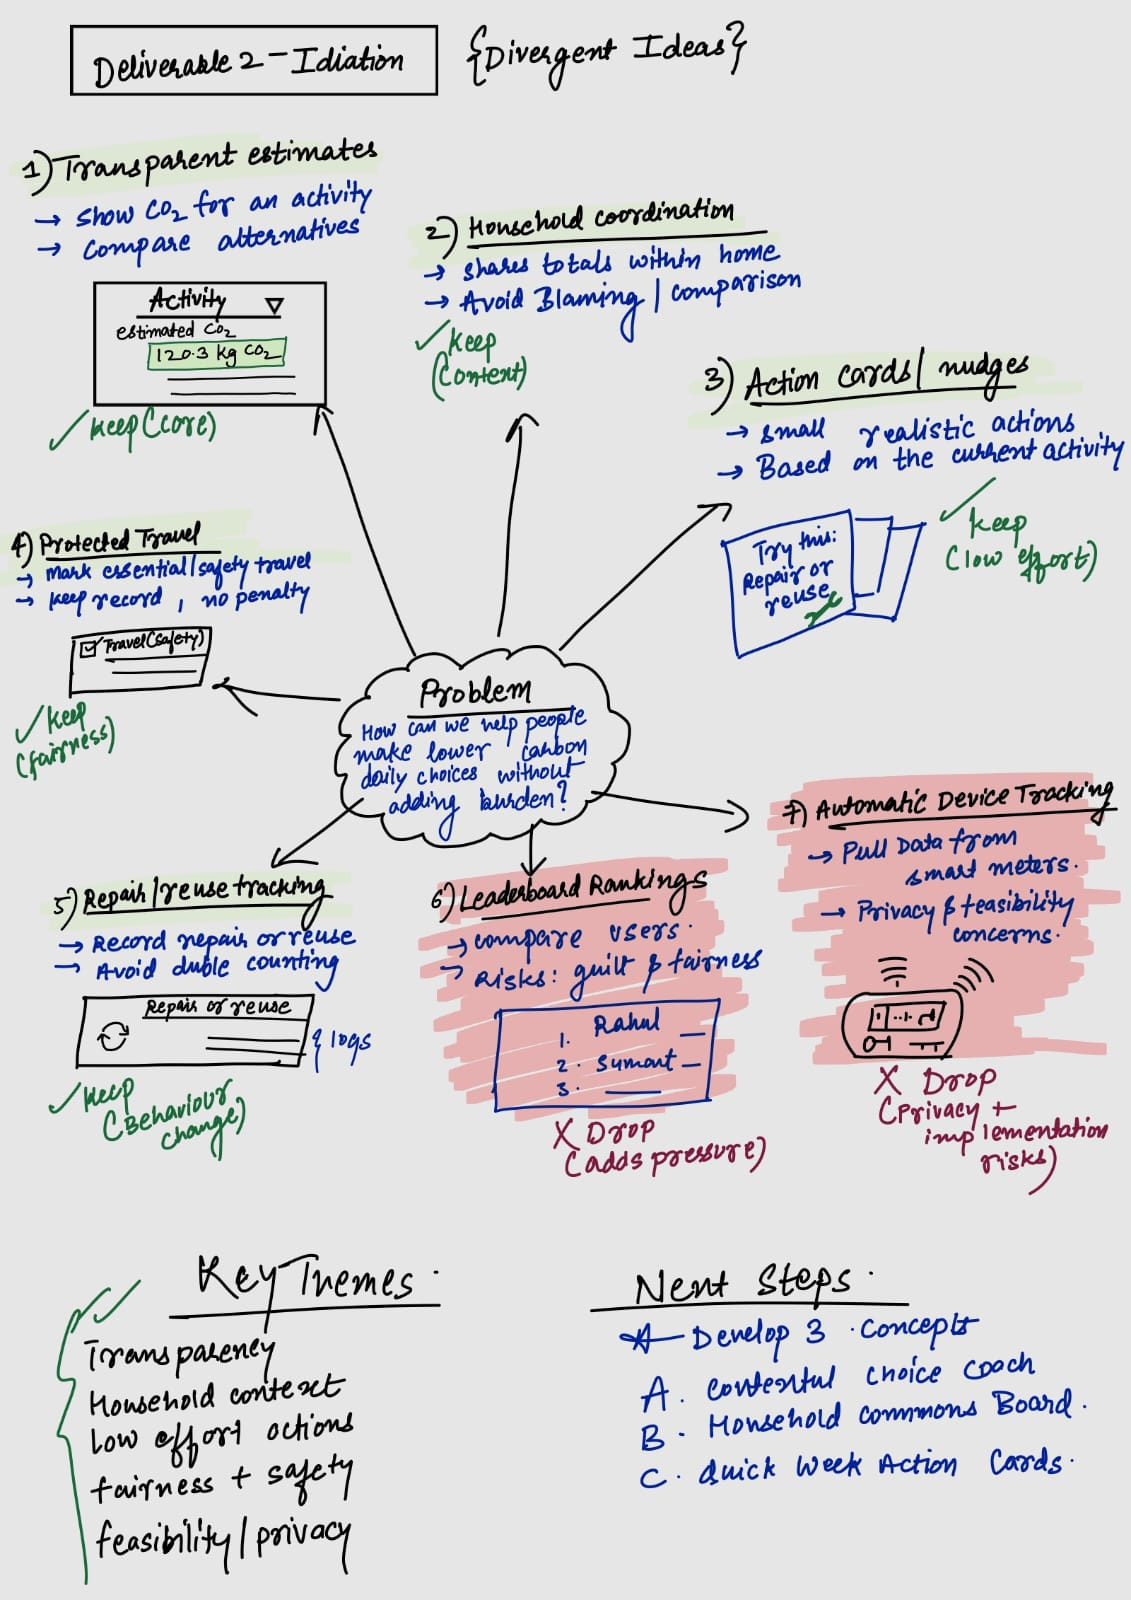
\includegraphics[width=\linewidth,height=5.6cm,keepaspectratio]{evidence/sketches/divergent.jpg}
\end{minipage}\hfill
\begin{minipage}[c]{0.66\textwidth}
\small
\textbf{Visible design exploration.} The annotated sheet places the D1 problem at the centre and tests transparent estimates, household coordination, action cards, protected journeys, repair/reuse, public rankings and automated tracking. The rejected directions are tied to pressure, fairness, privacy and implementation risk.\\[0.5em]
\textbf{Reading note.} These are illustrative working directions, not seven formally user-tested designs. The complete, zoomable source is reproduced in Appendix~\ref{fig:sketch_divergent}.
\end{minipage}
\caption{Team-supplied divergent-ideas sheet: a compact preview of decisions and rejected alternatives (full photograph: Appendix~\ref{fig:sketch_divergent}).}
\label{fig:divergent_preview}
\end{figure}

\Needspace{10\baselineskip}
\section{Three Distinct Conceptual Designs}

\begin{keybox}
\textbf{Sketch-to-concept evidence.} The annotated three-concept sheet (Appendix~\ref{fig:sketch_concepts}) illustrates the distinct interaction approaches compared below: \textbf{A}---an inspectable checkpoint journey, \textbf{B}---shared-home conversation and consent, and \textbf{C}---periodic, context-filtered cards. One concept sketch contains an inserted visual reference; it is presented as an annotated review sheet rather than a claim of wholly freehand contemporaneous ideation.
\end{keybox}

\Needspace{8\baselineskip}\subsection{Concept A: Contextual Choice Coach (Footprint Lens)}
\textbf{Interaction Paradigm:} \emph{Micro-decision checkpoint with contextual transparency.}

\begin{figure}[ht]
\centering
\begingroup
\hyphenpenalty=10000 \exhyphenpenalty=10000 % no hyphenation inside nodes
\resizebox{\linewidth}{!}{%
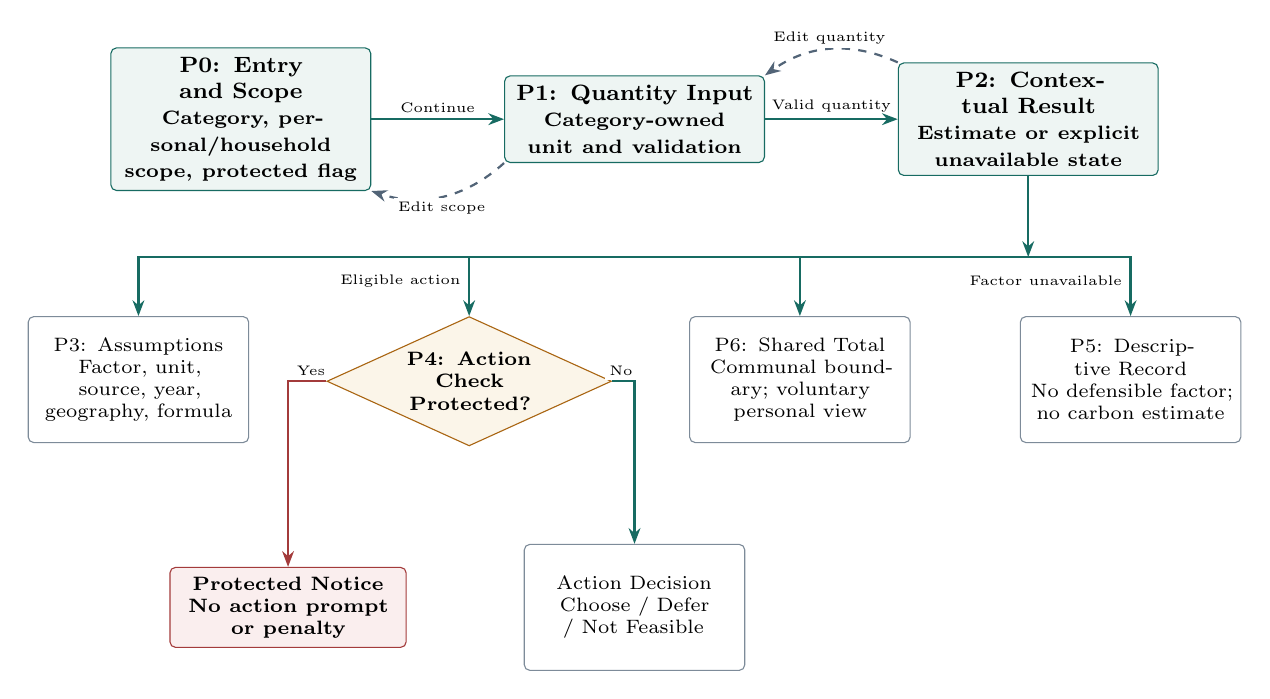
\begin{tikzpicture}[
  node distance=0.45cm and 0.45cm,
  main/.style={flowbox,align=center,minimum width=3.3cm,minimum height=1.1cm,text width=3.0cm},
  branch/.style={flowproc,align=center,minimum width=2.8cm,minimum height=1.6cm,text width=2.55cm},
  decision/.style={flowdec,align=center,inner sep=0pt,aspect=2.2,text width=2.0cm},
  safe/.style={flowalert,align=center,minimum width=3.0cm,minimum height=1.0cm,text width=2.75cm},
  arr/.style={flowarrow}, back/.style={backarrow},
  lbl/.style={font=\tiny,fill=white,inner sep=1.5pt}
]
% Primary capture-and-result path.
\node[main] (p0) at (-5.0,0) {P0: Entry and Scope\\{\scriptsize Category, personal/household scope, protected flag}};
\node[main] (p1) at (0,0) {P1: Quantity Input\\{\scriptsize Category-owned unit and validation}};
\node[main] (p2) at (5.0,0) {P2: Contextual Result\\{\scriptsize Estimate or explicit unavailable state}};
\draw[arr] (p0.east) -- node[above=1pt,font=\tiny,inner sep=1pt]{Continue} (p1.west);
\draw[arr] (p1.east) -- node[above=1pt,font=\tiny,inner sep=1pt]{Valid quantity} (p2.west);
\draw[back] (p1.south west) to[bend left=30] node[lbl,below]{Edit scope} (p0.south east);
\draw[back] (p2.north west) to[bend right=30] node[lbl,above]{Edit quantity} (p1.north east);

% Four optional routes: top-aligned, equal height.
\node[branch,anchor=north] (p3) at (-6.3,-2.5) {P3: Assumptions\\{\scriptsize Factor, unit, source, year, geography, formula}};
\node[decision,anchor=north] (p4) at (-2.1,-2.5) {P4: Action Check\\{\scriptsize Protected?}};
\node[branch,anchor=north] (p6) at (2.1,-2.5) {P6: Shared Total\\{\scriptsize Communal boundary; voluntary personal view}};
\node[branch,anchor=north] (p5) at (6.3,-2.5) {P5: Descriptive Record\\{\scriptsize No defensible factor; no carbon estimate}};

% Hub distributes P2 to the four optional routes.
\coordinate (hub) at (5.0,-1.75);
\draw[arr] (p2.south) -- (hub);
\draw[arr] (hub) -| (p3.north);
\draw[arr] (hub) -| (p4.north);
\draw[arr] (hub) -| (p6.north);
\draw[arr] (hub) -| (p5.north);
\node[lbl,anchor=east] at (-2.15,-2.05) {Eligible action};
\node[lbl,anchor=east] at (6.25,-2.05) {Factor unavailable};

% Outcomes of the action check, with clean orthogonal routing.
\node[safe] (protected) at (-4.4,-6.2) {Protected Notice\\{\scriptsize No action prompt or penalty}};
\node[branch] (action) at (0,-6.2) {Action Decision\\{\scriptsize Choose / Defer / Not Feasible}};
\draw[alertarrow] (p4.west) -| node[lbl,above,pos=0.2]{Yes} (protected.north);
\draw[arr] (p4.east) -| node[lbl,above,pos=0.2]{No} (action.north);
\end{tikzpicture}%
}
\endgroup
\caption{Professional Flowchart: Concept A Contextual Choice Coach Interaction Model}
\label{fig:concept_a_flow}
\end{figure}

\textbf{Mechanics \& Walkthrough:} Concept A (Figure~\ref{fig:concept_a_flow}) guides the user through single, bite-sized routine checkpoints. On P0, the user selects an activity, declares personal or household scope, and can flag the routine as \emph{protected}. On P1, quantity is entered with automatic unit ownership. On P2, the user receives an illustrative estimate alongside a familiar non-carbon contextual reference (e.g., INR electricity cost or 15-litre bucket counts). P2 acts as a universal router: users can inspect full data provenance (P3), consider an eligible action (P4), review the shared household boundary (P6), or view descriptive reasons for missing factors (P5).

\textbf{Persona Scenario (P4 Priya, Shift Worker):} Priya logs late-night safety-cab travel (15 km). Recognising night safety as non-negotiable, she checks ``Mark as protected''. Upon viewing P4, the system disables substitution demands (e.g., ``Take the bus'') and confirms: ``\emph{Action decisions are disabled because this activity is marked protected.}'' Priya receives a non-punitive confirmation rather than a reduction demand.

\Needspace{8\baselineskip}\subsection{Concept B: Household Commons Board}
\textbf{Interaction Paradigm:} \emph{Communal coordination and conversational consensus.}

\begin{figure}[ht]
\centering
\begingroup
\hyphenpenalty=10000 \exhyphenpenalty=10000 % no hyphenation inside nodes
\resizebox{\linewidth}{!}{%
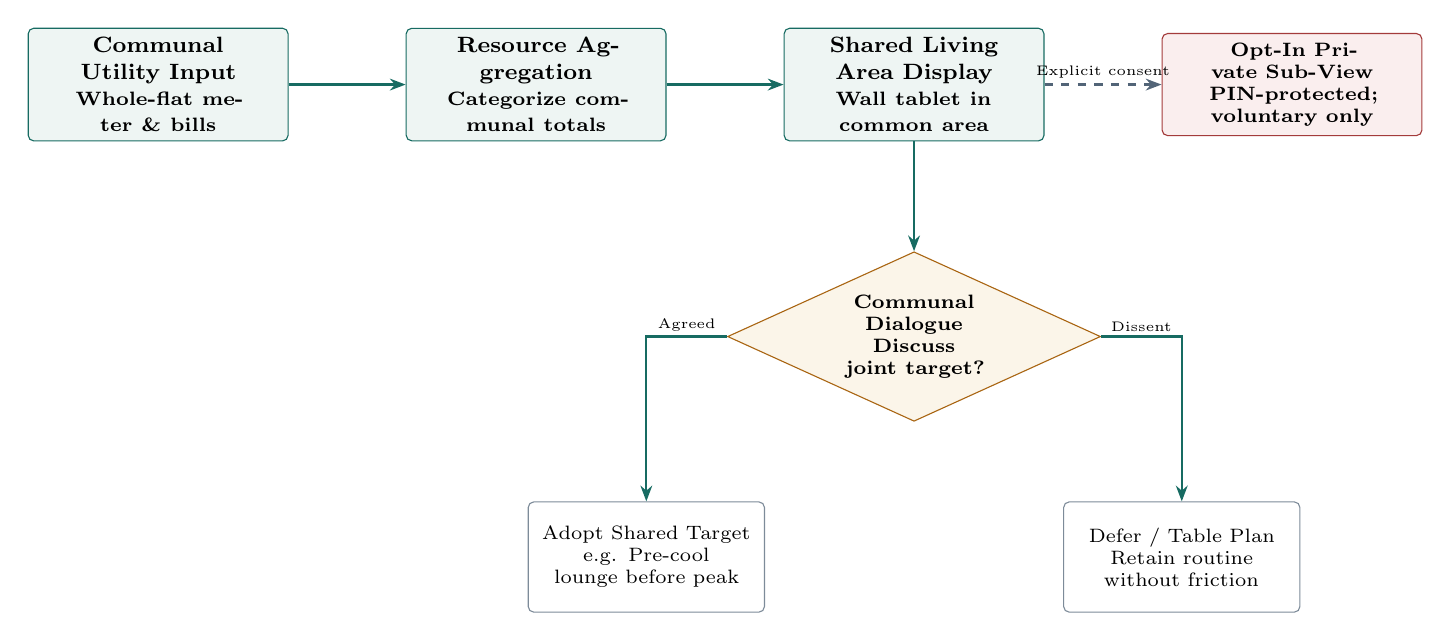
\begin{tikzpicture}[
  node distance=0.45cm and 0.45cm,
  main/.style={flowbox,align=center,minimum width=3.3cm,minimum height=1.1cm,text width=3.0cm},
  branch/.style={flowproc,align=center,minimum width=3.0cm,minimum height=1.4cm,text width=2.75cm},
  decision/.style={flowdec,align=center,inner sep=0pt,aspect=2.2,minimum width=3.6cm,text width=2.4cm},
  safe/.style={flowalert,align=center,minimum width=3.3cm,minimum height=1.1cm,text width=3.0cm},
  arr/.style={flowarrow}, back/.style={backarrow},
  lbl/.style={font=\tiny,fill=white,inner sep=1.5pt}
]
% Primary path across the top row.
\node[main] (meters) at (-4.8,0) {Communal Utility Input\\{\scriptsize Whole-flat meter \& bills}};
\node[main] (agg)    at (0,0)    {Resource Aggregation\\{\scriptsize Categorize communal totals}};
\node[main] (display) at (4.8,0) {Shared Living Area Display\\{\scriptsize Wall tablet in common area}};
\node[safe] (optin)  at (9.6,0)  {Opt-In Private Sub-View\\{\scriptsize PIN-protected; voluntary only}};

\draw[arr] (meters.east) -- (agg.west);
\draw[arr] (agg.east) -- (display.west);
\draw[back] (display.east) -- node[above=1pt,font=\tiny,inner sep=1pt]{Explicit consent} (optin.west);

% Dialogue checkpoint directly beneath the display.
\node[decision] (dialogue) at (4.8,-3.2) {Communal Dialogue\\{\scriptsize Discuss joint target?}};
\draw[arr] (display.south) -- (dialogue.north);

% Outcomes, level with each other.
\node[branch] (target) at (1.4,-6.0) {Adopt Shared Target\\{\scriptsize e.g. Pre-cool lounge before peak}};
\node[branch] (tabled) at (8.2,-6.0) {Defer / Table Plan\\{\scriptsize Retain routine without friction}};
\draw[arr] (dialogue.west) -| node[lbl,above,pos=0.25]{Agreed} (target.north);
\draw[arr] (dialogue.east) -| node[lbl,above,pos=0.25]{Dissent} (tabled.north);
\end{tikzpicture}%
}
\endgroup
\caption{Professional Flowchart: Concept B Household Commons Board Interaction Model}
\label{fig:concept_b_flow}
\end{figure}

\textbf{Mechanics \& Walkthrough:} Concept B (Figure~\ref{fig:concept_b_flow}) is designed for a shared tablet in communal living spaces. It aggregates whole-home utility data into shared resource cards (e.g., central geyser, water tanker delivery). Instead of individual scorecards, it presents joint action proposals for household discussion. Individual personal views are strictly opt-in and pin-protected to prevent flatmates or parents from policing each other.

\textbf{Persona Scenario (P1 Ananya, Student Hostel):} Ananya lives in a shared student accommodation context. They share a central geyser and refrigerator. Concept B displays the communal 320 kWh bill. Instead of attempting to divide the bill into four fraught individual shares, the display suggests: ``\emph{Shift geyser heating 30 minutes earlier to utilize solar grid hours.}'' The flatmates agree over dinner without interpersonal conflict.

\Needspace{8\baselineskip}\subsection{Concept C: Quiet-Week Action Cards}
\textbf{Interaction Paradigm:} \emph{Constraint-first asynchronous nudges.}

\begin{figure}[ht]
\centering
\begingroup
\hyphenpenalty=10000 \exhyphenpenalty=10000 % no hyphenation inside nodes
\resizebox{\linewidth}{!}{%
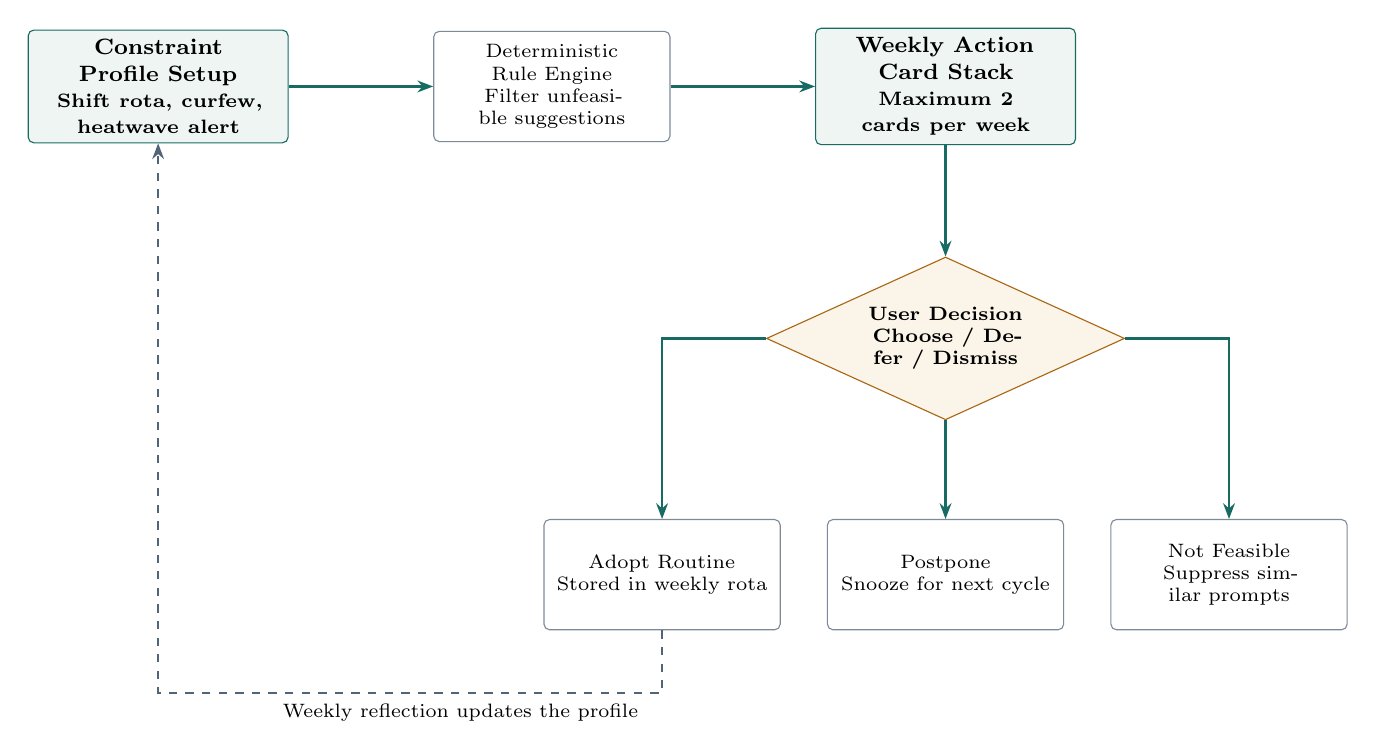
\begin{tikzpicture}[
  node distance=0.45cm and 0.45cm,
  main/.style={flowbox,align=center,minimum width=3.3cm,minimum height=1.1cm,text width=3.0cm},
  branch/.style={flowproc,align=center,minimum width=3.0cm,minimum height=1.4cm,text width=2.75cm},
  decision/.style={flowdec,align=center,inner sep=0pt,aspect=2.2,minimum width=4.2cm,text width=2.8cm},
  arr/.style={flowarrow}, back/.style={backarrow},
  lbl/.style={font=\tiny,fill=white,inner sep=1.5pt}
]
% Primary path across the top row.
\node[main]   (filter) at (-5.0,0) {Constraint Profile Setup\\{\scriptsize Shift rota, curfew, heatwave alert}};
\node[branch] (engine) at (0,0)    {Deterministic Rule Engine\\{\scriptsize Filter unfeasible suggestions}};
\node[main]   (cards)  at (5.0,0)  {Weekly Action Card Stack\\{\scriptsize Maximum 2 cards per week}};
\draw[arr] (filter.east) -- (engine.west);
\draw[arr] (engine.east) -- (cards.west);

% Decision checkpoint directly beneath the card stack.
\node[decision] (decision) at (5.0,-3.2) {User Decision\\{\scriptsize Choose / Defer / Dismiss}};
\draw[arr] (cards.south) -- (decision.north);

% Outcomes on one level.
\node[branch] (accept)  at (1.4,-6.2) {Adopt Routine\\{\scriptsize Stored in weekly rota}};
\node[branch] (defer)   at (5.0,-6.2) {Postpone\\{\scriptsize Snooze for next cycle}};
\node[branch] (dismiss) at (8.6,-6.2) {Not Feasible\\{\scriptsize Suppress similar prompts}};
\draw[arr] (decision.west) -| (accept.north);
\draw[arr] (decision.south) -- (defer.north);
\draw[arr] (decision.east) -| (dismiss.north);

% Feedback loop routed below the outcome row, clear of all boxes.
\draw[back] (accept.south) -- ++(0,-0.8) -| node[lbl,font=\scriptsize,below=2pt,pos=0.2]{Weekly reflection updates the profile} (filter.south);
\end{tikzpicture}%
}
\endgroup
\caption{Professional Flowchart: Concept C Quiet-Week Action Cards Interaction Model}
\label{fig:concept_c_flow}
\end{figure}

\textbf{Mechanics \& Walkthrough:} Concept C (Figure~\ref{fig:concept_c_flow}) eliminates continuous daily logging. The user inputs their external operational constraints once. The system suppresses daily prompts and delivers a maximum of two inspectable, rule-based recommendation cards per week. Cards explicitly declare why they were selected and allow users to accept, postpone, or dismiss without penalty.

\textbf{Persona Scenario (P5 Sunita, Household Manager):} During peak summer, Sunita inputs heatwave constraints. Concept C delivers one card: ``\emph{Use residual microwave heat for evening defrosting rather than running the tap.}'' Sunita accepts it with one tap; the app sleeps for the rest of the week, respecting her busy schedule.

\Needspace{10\baselineskip}
\section{Concept Selection and Novelty Analysis}

\begin{chapterfocus}{Three candidates, three interaction logics}
\vspace{-0.9em}
\renewcommand{\arraystretch}{1}
\setlength{\parskip}{0pt}
\setlength{\tabcolsep}{0pt}
\begin{tabularx}{\linewidth}{@{}X@{\hspace{12pt}}X@{\hspace{12pt}}X@{}}
{\sffamily\bfseries\color{Teal}A\enspace}{\bfseries\color{Navy}Checkpoint coach}\par\vspace{1pt}
{\small\color{Slate}Immediate, auditable decision flow.}
&
{\sffamily\bfseries\color{Teal}B\enspace}{\bfseries\color{Navy}Commons board}\par\vspace{1pt}
{\small\color{Slate}Group-level coordination with consent risks.}
&
{\sffamily\bfseries\color{Teal}C\enspace}{\bfseries\color{Navy}Quiet cards}\par\vspace{1pt}
{\small\color{Slate}Low effort, but delayed and less directly evidenced feedback.}
\end{tabularx}
\par\vspace{0.5em}
{\color{RuleGray}\rule{\linewidth}{0.5pt}}\par\vspace{0.35em}
{\small\itshape The decision is about interaction architecture, not visual preference.}
\vspace{-0.6em}
\end{chapterfocus}

\begin{keybox}
\textbf{Refinement evidence.} Appendix~\ref{fig:sketch_refinement} shows the Concept A screen sketches, accepted trade-offs and unresolved questions. The drawing places P3 and P4 in a simple left-to-right sequence for discussion; the \emph{final} user journey correctly branches from the P2 result hub, as specified in Figure~\ref{fig:concept_a_flow} and the Figma walkthrough. This distinction makes the progression from a rough sketch to the revised flow explicit.
\end{keybox}

\subsection{Multi-Criteria Evaluation Matrix}
To determine the single concept for prototype implementation, the three models were evaluated across five weighted engineering and stakeholder criteria derived from the rubric:

\begin{table}[ht]
\centering
\small
\caption{Weighted multi-criteria decision analysis (working ratings; 1--5 scale).}
\label{tab:mcdm}
\begin{tabularx}{\textwidth}{@{}>{\raggedright\arraybackslash}X>{\centering\arraybackslash}p{1.35cm}>{\centering\arraybackslash}p{2.38cm}>{\centering\arraybackslash}p{2.38cm}>{\centering\arraybackslash}p{2.38cm}@{}}
\toprule
\textbf{Criterion} & \textbf{Weight} & \textbf{A: Choice Coach} & \textbf{B: Commons Board} & \textbf{C: Quiet Cards}\\
\midrule
D1 Must-Have coverage (E1--E5) & 25\% & 5.0 & 3.0 & 3.0\\
Persona and scenario fit (P1--P6; SC1--SC4) & 25\% & 4.5 & 4.0 & 3.5\\
Implementation feasibility (bounded offline prototype) & 20\% & 5.0 & 2.5 & 3.5\\
Transparency and provenance & 15\% & 5.0 & 3.0 & 2.5\\
Socio-technical risk profile & 15\% & 4.5 & 2.0 & 3.0\\
\midrule
\textbf{Weighted score} & \textbf{100\%} & \textbf{4.80/5} & \textbf{3.00/5} & \textbf{3.15/5}\\
\bottomrule
\end{tabularx}
\end{table}

\textbf{Scoring anchors.} Ratings use an ordinal five-point scale: 1 = material conflict with the criterion; 2 = substantial gaps; 3 = partial coverage with significant limitations; 4 = good coverage with manageable limitations; 5 = strong conceptual alignment with no major gap identified. A feasibility score assesses whether the concept can be represented within the proposed project scope; it is not evidence that implementation has been completed. Weighted totals are calculated as $\sum_i w_i s_i$ with weights summing to 1. The ratings are provisional design judgements requiring team sign-off, not empirical usability results.

\begin{insightbox}{Design decision | Select Concept A: Contextual Choice Coach}
Concept A integrates quick activity capture (E1/E5), visible evidence and assumptions (E2), constraint-aware decisions (E3), and honest treatment of unsupported categories (E4) in a single inspectable journey. The shared-versus-personal boundary remains explicit. Its weighted design score is \textbf{4.80/5}, compared with 3.15/5 for the next-highest alternative; this is a working decision matrix, not a user preference study.
\end{insightbox}

\textbf{Trade-off.} Concept B offers richer household coordination but introduces consent and visibility risks; Concept C demands less entry effort but separates action cards from the immediate calculation evidence. Concept A still requires a usability check: manual entry could feel burdensome, and users may misread provisional emissions factors as verified.

\textbf{Sensitivity and limits.} On the declared weights, A scores 4.80/5 versus 3.15/5 for the closest alternative C. This lead follows from the working judgements on Must-Have coverage and inspectable evidence; changing those assumptions could change the choice. The ratings are not user preference data. A also has risks of additional manual input and misunderstood provisional factors, which the low-fidelity evaluation must explicitly test.

\subsection{Key Design Decision Log}
The selection is more useful when its consequences are made explicit. The following decision log records the principal trade-offs carried into the selected concept; it is a design rationale, not a claim that the alternatives were empirically tested.

\begin{table}[ht]
\centering
\small
\caption{Design decision log for the selected Concept A}
\label{tab:decision-log}
\begin{tabularx}{\textwidth}{@{}>{\raggedright\arraybackslash}p{2.45cm}>{\raggedright\arraybackslash}p{3.0cm}>{\raggedright\arraybackslash}X>{\raggedright\arraybackslash}p{2.5cm}@{}}
\toprule
\textbf{Decision} & \textbf{Alternative considered} & \textbf{Rationale for selected approach} & \textbf{Consequence}\\
\midrule
Manual, local entry & Automated bill/order ingestion & Avoids account access, brittle parsing and cloud dependencies; preserves user control over the quantity entered. & More user effort; lower privacy exposure.\\
\rowcolor{brandlight}
Protected routine state & Uniform reduction prompts & Safety, medical and shift constraints are not discretionary optimisation targets. & P4 suppresses action prompts for protected routines.\\
Communal default & Automatic per-person bill division & Shared meters do not establish individual consumption. & P6 shows communal totals; attribution is voluntary and bounded.\\
\rowcolor{brandlight}
Descriptive unknown state & Estimated offset for every habit & Unsupported factors would create false precision. & P5 preserves the activity record without a numeric credit.\\
Progressive disclosure & One dense dashboard & A simple primary journey and a separate audit route serve different information needs. & P2 remains the hub; P3 contains technical detail.\\
\bottomrule
\end{tabularx}
\end{table}

\subsection{Novelty and Competitor Comparison}
The coursework requires a design that is not substantially the same as an existing commercial product \cite{modulebrief}. Carbon calculators and action tools already exist: Earth Hero publicly describes footprint tracking and climate actions; Giki Zero is described as a personalised tool for understanding, tracking and reducing one's footprint \cite{earthhero,gikizero}. The product descriptions do not permit a reliable claim that competitors \emph{lack} a feature. Table~\ref{tab:competitor} therefore compares their documented emphasis with the \emph{proposed} Footprint Lens interaction contract rather than asserting exclusivity.

\begin{table}[ht]
\centering\small
\caption{Evidence-bounded differentiation: documented product positioning versus the proposed integrated flow.}
\label{tab:competitor}
\begin{tabularx}{\textwidth}{@{}p{2.75cm}XX@{}}
\toprule
\textbf{Dimension}&\textbf{Publicly described comparator capabilities}&\textbf{Specific Footprint Lens design decision}\\
\midrule
Footprint and actions&Earth Hero promotes footprint tracking and accessible climate actions; Giki Zero promotes a calculator and practical reduction steps.&P2 links one recorded activity to its estimate and directly to P3 evidence and P4 feasible action, rather than just a score.\\
\rowcolor{RowGray}
Evidence provenance&The published product summaries do not establish the granularity of factor editing or local-source metadata in every product version.&P3 explicitly exposes quantity, units, provisional source, geography, year status and formula; user edits must remain identifiable.\\
Safety constraints&The cited summaries do not demonstrate a dedicated safety-locked branch for night-shift travel, heat and hostel curfews.&P0's protected flag determines P4's advice eligibility, without changing the underlying footprint arithmetic.\\
\rowcolor{RowGray}
Shared-home accountability&Neither a public product summary nor a footprint total is sufficient to infer an individual flatmate's measured share.&P6 uses communal totals by default; any own-room attribution requires independent input and explicit opt-in.\\
Unsupported categories&No tool should be assumed to have a credible factor for every repair, packaging or waste activity.&P2/P5 label such results ``unavailable'' and preserve descriptions without false avoided-emission credits.\\
\bottomrule
\end{tabularx}
\end{table}

\begin{insightbox}{Differentiation to test, not market exclusivity}
\textbf{Transparent calculation checkpoint} $\rightarrow$ \textbf{constraint-aware, non-punitive choice} $\rightarrow$ \textbf{shared-home consent boundary}. These three mechanisms form the proposed integrated contribution. The cited product descriptions cannot establish exclusive novelty or substitute for a competitor usability study.
\end{insightbox}

% Previous section content ends here.
\clearpage
% New section content starts here.
\section{Small User Stories and MoSCoW Prioritisation}

\begin{chapterfocus}{Backlog reading guide}
\vspace{-1.4em}
\renewcommand{\arraystretch}{1}
\setlength{\parskip}{0pt}
\setlength{\tabcolsep}{0pt}
\begin{tabularx}{\linewidth}{@{}X@{\hspace{12pt}}X@{\hspace{12pt}}X@{}}
{\sffamily\bfseries\color{Teal}1\enspace}{\bfseries\color{Navy}Parent stories}\par\vspace{1pt}
{\small\color{Slate}US01--US14 preserve D1 identity and original MoSCoW decisions.}
&
{\sffamily\bfseries\color{Teal}2\enspace}{\bfseries\color{Navy}Child stories}\par\vspace{1pt}
{\small\color{Slate}Implementation-sized units below, proposed for acceptance testing.}
&
{\sffamily\bfseries\color{Teal}3\enspace}{\bfseries\color{Navy}Won't Have}\par\vspace{1pt}
{\small\color{Slate}Epics E13--E14 remain release guards, not feature promises.}
\end{tabularx}
\par\vspace{0.5em}
{\color{RuleGray}\rule{\linewidth}{0.5pt}}\par\vspace{0.35em}
{\small\itshape Each child inherits its parent epic, personas, scenarios and priority; no D1 epic is silently reprioritised.}
\vspace{-0.9em}
\end{chapterfocus}


The story register translates the D1 requirements baseline into a traceable backlog for the selected Contextual Choice Coach. It retains the original epic identifiers and priority decisions: E1--E5 are Must Have, E6--E9 are Should Have, E10--E12 are Could Have, and E13--E14 are Won't Have in v1.0. This preserves continuity between the problem definition, conceptual design and subsequent implementation planning.

The D1 persona identifiers are retained throughout: P1 Ananya Deshmukh, P2 Karthik Sundaram, P3 Rohan Kulkarni, P4 Priya Reddy, P5 Sunita Sharma and P6 Rajeshwar Prasad Verma. Scenario references SC1--SC4 also retain their D1 meanings. Each story states the stakeholder outcome first, then gives observable Given/When/Then acceptance criteria. These criteria specify intended behaviour; they are not claims that every capability has already been implemented or evaluated.

The sequence is deliberately layered. Must-have stories establish the minimum trustworthy interaction: capture a routine, explain its estimate and assumptions, protect constrained activities, acknowledge circular practices honestly, and support brief offline entry. Should-have stories add comparison, shared-household boundaries, summaries and researcher export. Could-have stories extend the experience with rota-aware timing, benchmarks and locally stored plans. Won't-have stories make explicit which forms of surveillance, coercive attribution and unsupported automation are excluded.

\begin{storybox}{US01 (Epic E1): Tangible Dual-Unit Metric Translation}{MoSCoW: Must Have | Personas: P1, P3, P5, P6 | Scenarios: SC1, SC2, SC4}
\textbf{User Story:} As an urban Indian user unfamiliar with abstract climate metrics, I want an estimate accompanied by relevant, clearly labelled everyday measures where defensible (Indian Rupees, 15-litre water buckets, fan/AC hours, and city bus trips) alongside $\text{kg CO}_2$, so that I can immediately picture the real-world scale of my household and commuting routines.
\begin{itemize}
    \item \textbf{Given} a valid routine quantity is entered or selected via preset in State P1 (e.g., $168.0\text{ kWh}$ monthly electricity),
    \item \textbf{When} the calculation engine executes the emission conversion strategy,
    \item \textbf{Then} State P2 displays the illustrative electricity result ($120.29\text{ kg CO}_2$) beside the assumed electricity cost (Rs. 1,344). The interface labels the factor as provisional and does not imply that water volume or currency is a carbon equivalent.
\end{itemize}
\end{storybox}

\begin{storybox}{US02 (Epic E2): Transparent Assumption Inspection and Live Editing}{MoSCoW: Must Have | Personas: P2, P3, P5, P6 | Scenarios: SC1--SC4}
\textbf{User Story:} As an evidence-conscious researcher or analytical householder, I want to inspect and edit the underlying conversion assumptions (electricity grid-emission factor, electricity tariff rate, and mathematical formula), so that I can verify where estimates come from and calibrate them to my state electricity board bill.
\begin{itemize}
    \item \textbf{Given} a calculated routine footprint in State P2,
    \item \textbf{When} the user opens the assumptions panel and changes an editable illustrative parameter (for example, the grid factor or tariff),
    \item \textbf{Then} the interface displays the revised formula and recalculated estimate, while retaining the parameter's unit, source, geography, reference year, and provisional status.
\end{itemize}
\end{storybox}

\begin{storybox}{US03 (Epic E3): Structural Constraint Shield for Safety and Shift Routines}{MoSCoW: Must Have | Personas: P1, P3, P4 | Scenarios: SC2--SC4}
\textbf{User Story:} As a user whose routine is constrained by safety, health, housing, or work conditions, I want to flag non-negotiable activities (such as a night-shift safety cab, essential cooling during daytime sleep, or a hostel curfew constraint), so that the tool does not frame an infeasible change as a personal failure.
\begin{itemize}
    \item \textbf{Given} the user checks the \textit{Protected Health/Safety Routine} checkbox in State P0,
    \item \textbf{When} the user views the Constraint Shield action screen in State P4,
    \item \textbf{Then} the protected routine is visibly labelled \textit{Protected}; no reduction prompt, negative score, or penalty is displayed for it. Optional actions remain available only for routines not marked as protected.
\end{itemize}
\end{storybox}

\begin{storybox}{US04 (Epic E4): Descriptive Circularity and Low-Waste Habit Recognition}{MoSCoW: Must Have | Personas: P1--P6 | Scenarios: SC1--SC4}
\textbf{User Story:} As a user practising lower-waste and circular activities, I want relevant actions (including repair and longer product use, composting, recycling, food-waste reduction, reusable packaging, and lower-waste food or clothing choices) recorded honestly, so that the tool recognises these practices without inventing unsupported carbon savings.
\begin{itemize}
    \item \textbf{Given} the user selects a supported circularity or lower-waste category (for example, repair, composting, recycling, food-waste reduction, or reusable packaging) in State P5,
    \item \textbf{When} the habit is saved with the optional descriptive-summary setting selected,
    \item \textbf{Then} the system logs the practice as a descriptive record (not a verified environmental-impact claim) explicitly labelled \textit{Status: Estimate Unavailable (No Fake Offsets)} and never subtracts fabricated $\text{kg CO}_2$ deductions from direct energy totals.
\end{itemize}
\end{storybox}

\begin{storybox}{US05 (Epic E5): Offline 2-Tap Preset Logger and Plain Hindi Toggle}{MoSCoW: Must Have | Personas: P1, P2, P4, P5, P6 | Scenarios: SC1--SC4}
\textbf{User Story:} As a time-poor user who may have limited connectivity or prefer a familiar language, I want routine presets and an English / Plain Hindi interface that remains usable offline, with relevant local-language guidance cards for the contexts identified in D1, so that I can record a routine with minimal effort.
\begin{itemize}
    \item \textbf{Given} the application is running with zero network connectivity,
    \item \textbf{When} the user has completed initial language and scope setup and selects one preset in State P1,
    \item \textbf{Then} the selected preset fills its quantity and unit and can be submitted without a network connection. The design target is no more than two logging actions and 60 seconds for a familiar preset task; both measures are evaluated rather than assumed. English and Plain Hindi are the initial interface options; additional language cards identified in D1 for SC2 and SC4 are content extensions, not a claim of complete interface localisation.
\end{itemize}
\end{storybox}

\begin{insightbox}{Minimum credible journey | Must-Have E1--E5}
Together, US01--US05 define the minimum credible loop. A resident begins with a familiar activity and a clear personal or household boundary; the system accepts a valid quantity and presents an estimate only where a defensible factor exists. The user can inspect the assumptions behind that estimate, mark an unavoidable routine as protected, or record a circular practice without receiving a fabricated carbon credit. Offline presets and plain-language entry reduce the effort required to repeat this loop. These stories address both sides of the D1 problem: understanding the number and ensuring that the suggested response respects real living conditions.
\end{insightbox}

\begin{storybox}{US06 (Epic E6): Side-by-Side What-If Habit Swap Simulator}{MoSCoW: Should Have | Personas: P1, P3, P5 | Scenarios: SC1, SC2, SC4}
\textbf{User Story:} As a decision-maker comparing everyday alternatives, I want an interactive What-If slider that previews the estimated changes in Rupee cost and emissions of a realistic adjustment (such as cutting WFH AC runtime by 1 hour or swapping one car commute to the Metro), so that I can evaluate trade-offs before committing.
\begin{itemize}
    \item \textbf{Given} a baseline routine calculation in State P2 ($168.0\text{ kWh} = 120.29\text{ kg CO}_2$ using the provisional D1 assumption),
    \item \textbf{When} the user adjusts the \textit{What-If Swap Simulator} slider (\textit{Cut 1.5 kW WFH AC 1 hr early}),
    \item \textbf{Then} the simulator displays the estimated difference beside the baseline and exposes the assumptions used. Under the D1 illustrative assumptions (1.5 kW, one hour, 14 days, 0.716 kg CO$_2$/kWh, Rs. 8/kWh), the example is 21 kWh, approximately 15.04 kg CO$_2$, and Rs. 168 in variable electricity cost. These are scenario outputs, not guaranteed savings, and the grid factor remains provisional.
\end{itemize}
\end{storybox}

\begin{storybox}{US07 (Epic E7): Shared Household Boundary with Voluntary Opt-In}{MoSCoW: Should Have | Personas: P1, P2, P3, P5, P6 | Scenarios: SC1, SC2, SC4}
\textbf{User Story:} As a resident in a multi-generational home or shared student flat, I want shared utility bills displayed as a communal total by default with a strictly voluntary opt-in toggle for my own room share, so that we can coordinate household reductions without policing or blaming flatmates.
\begin{itemize}
    \item \textbf{Given} \textit{Household Scope} is selected for a shared bill ($168\text{ kWh}$) in State P6,
    \item \textbf{When} the Shared Household Boundary view loads,
    \item \textbf{Then} it displays the \textit{Communal Total (Default)} and the rule \textit{``Shared bills do not equal personal footprints''}; only the active user can opt in to displaying their own share, and no other resident's usage is inferred or exposed without consent.
\end{itemize}
\end{storybox}

\begin{storybox}{US08 (Epic E8): Non-Judgmental Monthly Summary and Single Challenge}{MoSCoW: Should Have | Personas: P1, P3, P5 | Scenarios: SC2, SC4}
\textbf{User Story:} As a user fatigued by moralising eco-guilt, I want a clean monthly category breakdown paired with a single optional monthly challenge (such as keeping a smartphone an extra year or batching grocery orders), so that I can track progress without punitive streak counters.
\begin{itemize}
    \item \textbf{Given} the user has logged one or more routines during the selected calendar month,
    \item \textbf{When} the monthly summary is viewed,
    \item \textbf{Then} the summary shows the selected month, groups available records by domain (Energy, Mobility, Delivery/Packaging, Circularity), and distinguishes unavailable estimates from zero impact. If no records exist, it displays an empty state inviting the user to add a record. No leaderboard, punitive streak, or negative personal score is shown.
\end{itemize}
\end{storybox}

\begin{storybox}{US09 (Epic E9): Researcher Audit View and Local CSV Export}{MoSCoW: Should Have | Personas: P2 | Scenario: SC4}
\textbf{User Story:} As an environmental science postgraduate, I want to export session logs and active assumption parameters to a local CSV file, so that I can perform regional sensitivity analyses in external research tools without cloud dependencies.
\begin{itemize}
    \item \textbf{Given} active session calculations and provenance parameters in State P3,
    \item \textbf{When} the user clicks \textit{Export CSV Data},
    \item \textbf{Then} in the planned Increment 2 implementation, the system writes a structured \texttt{.csv} file containing quantities, units, grid factors, tariffs, and calculated $\text{kg CO}_2$ directly to the local filesystem.
\end{itemize}
\end{storybox}

\paragraph{Should-have extension (E6--E9).}
Once the core loop is trustworthy, US06--US09 extend it from individual understanding to informed decision-making and household coordination. The What-If comparison supports deliberation rather than prescribing a single action; the shared-boundary view prevents a communal bill from being misrepresented as an individual's footprint; and the monthly summary supports reflection without leaderboards or punitive streaks. Researcher audit/export is deliberately deferred to Increment 2, keeping the first release focused on the simpler user journey.

\begin{storybox}{US10 (Epic E10): Rota Quiet Windows}{MoSCoW: Could Have | Personas: P4 | Scenario: SC3}
\textbf{User Story:} As a rotating night-shift worker, I want to configure a weekly quiet window aligned with my daytime sleep, so that optional feedback does not disturb my rest.
\begin{itemize}
    \item \textbf{Given} P4 Priya enables rota-aware quiet hours and enters her usual sleep window,
    \item \textbf{When} an optional reminder would otherwise be presented during that configured window,
    \item \textbf{Then} the reminder is suppressed during the quiet window, and the setting can be reviewed or disabled by the user. The feature does not infer a rota or send notifications in v1.0 unless separately implemented and tested.
\end{itemize}
\end{storybox}


\begin{storybox}{US11 (Epic E11): Static Reference-Flat Benchmark}{MoSCoW: Could Have | Personas: P3 | Scenario: SC4}
\textbf{User Story:} As a user surprised by my electricity bill, I want to compare my recorded household usage with a clearly described reference-flat range, so that I can interpret the figure without treating a benchmark as a personal target.
\begin{itemize}
    \item \textbf{Given} the user opens the optional benchmark view,
    \item \textbf{When} they select a flat-size reference category,
    \item \textbf{Then} the tool displays the reference range, source or derivation, location, period, and limitations; it does not claim that the range represents every household.
\end{itemize}
\end{storybox}

\begin{storybox}{US12 (Epic E12): Record a Smart-Plug Timer Plan}{MoSCoW: Could Have | Personas: P3, P5 | Scenarios: SC1, SC4}
\textbf{User Story:} As a user who already owns a compatible smart plug, I want to record a planned appliance cut-off time, so that I can remember and review a proposed routine change without requiring a cloud hardware integration.
\begin{itemize}
    \item \textbf{Given} the user records a timer plan for a geyser or AC,
    \item \textbf{When} they save the plan,
    \item \textbf{Then} the application stores the schedule locally as a reminder/plan only and does not claim to control the physical device.
\end{itemize}
\end{storybox}

\paragraph{Could-have extensions (E10--E12).}
US10--US12 are valuable but not prerequisites for a coherent first release. Rota-aware quiet windows address the specific needs of P4 Priya in SC3; a static reference-flat benchmark supports interpretation for P3 Rohan in SC4; and a local smart-plug timer plan helps users remember a proposed change without pretending that the application controls physical hardware. Their lower priority protects implementation scope while preserving a clear path for later increments.

\begin{storybox}{US13 (Epic E13): No Public Rankings or Forced Attribution}{MoSCoW: Won't Have (v1.0) | Personas: All (P1--P6) | Scenarios: SC1--SC4}
\textbf{Excluded capability:} Public competitive leaderboards, mandatory per-person bill splitting without consent, individual rankings on communal displays, and punitive red scores are excluded. The product may show a household total, but it must not infer or disclose another resident's personal share. This preserves the consent boundary defined by D1 Epic E13 (\textbf{L1, L2, RQ3}).
\end{storybox}

\Needspace{18\baselineskip}
\begin{storybox}{US14 (Epic E14): No Unverified Automated Data or Offset Claims}{MoSCoW: Won't Have (v1.0) | Personas: All (P1--P6) | Scenarios: SC1--SC4}
\textbf{Excluded capability:} Live bank or credit-card scraping, cloud-based food-photo estimation, automatic hardware telemetry, building-material lifecycle claims without defensible data, and commercial offset marketplace integration are excluded from v1.0. Estimates must expose their factors and boundaries; where a defensible factor is unavailable, the system records the activity descriptively rather than fabricating a saving or offset. This is a v1.0 scope boundary, not a claim that every future version must remain permanently offline.
\end{storybox}

\paragraph{Explicit exclusions (E13--E14).}
The final two stories are boundary conditions, not deferred promises. E13 excludes public rankings and forced personal attribution because these would undermine consent and could turn shared tracking into household surveillance. E14 excludes unverified automated data collection and offset claims because a confident-looking number is not trustworthy without a defensible source, unit and system boundary. If an activity cannot be estimated responsibly, the product should preserve the descriptive record and state the limitation.

\Needspace{7\baselineskip}

% =========================================================================
% SMALL STORIES: VERIFICATION SLICES
% =========================================================================


\subsection{Small, Independently Testable Child Stories}
The original US01--US14 entries above are preserved as traceable D1-linked \emph{parent outcomes}. Table~\ref{tab:atomic-stories} is the actionable implementation backlog: each child has a single outcome, an inherited MoSCoW priority, and a distinct acceptance observation. This prevents large stories (especially US02 and US05) from being mistaken for independently deliverable tasks. The separate illustrative Figma states do not imply a functioning calculator, bilingual application or persistent storage.

\begin{chapterfocus}{Acceptance design rule}
\vspace{-0.6em}
\renewcommand{\arraystretch}{1}
\setlength{\parskip}{0pt}
\setlength{\tabcolsep}{0pt}
\vspace{-0.6em}
\begin{tabularx}{\linewidth}{@{}X@{\hspace{12pt}}X@{\hspace{12pt}}X@{}}
{\sffamily\bfseries\color{Teal}1\enspace}{\bfseries\color{Navy}Figma example}\par\vspace{1pt}
{\small\color{Slate}The observable state is shown in the linked prototype.}
&
{\sffamily\bfseries\color{Teal}2\enspace}{\bfseries\color{Navy}Logic check}\par\vspace{1pt}
{\small\color{Slate}The rule is verified against the specified behaviour.}
&
{\sffamily\bfseries\color{Teal}3\enspace}{\bfseries\color{Navy}Future functional test}\par\vspace{1pt}
{\small\color{Slate}Confirmed only once the feature is built and run.}
\end{tabularx}
\par\vspace{0.5em}
{\color{RuleGray}\rule{\linewidth}{0.5pt}}\par\vspace{0.35em}
{\small\itshape Each child is checked independently. A pass requires the observable state shown in the acceptance condition; the final column marks which level of evidence applies, and these levels are not equivalent.}
\vspace{-0.6em}
\end{chapterfocus}

\begingroup
\footnotesize
\renewcommand{\arraystretch}{1.3}
\setlength{\tabcolsep}{4pt}
\rowcolors{2}{white}{RowGray!70}
\newcommand{\hdr}[1]{{\sffamily\bfseries\footnotesize\color{Navy}#1}}
% \story{parent}{priority}{child}{outcome title}{acceptance check}{evidence}
\newcommand{\story}[6]{%
  {\sffamily\bfseries\color{Navy}#1}\newline{\scriptsize\color{Slate}#2} &
  {\sffamily\bfseries\color{Teal}#3} &
  \textbf{#4} #5 &
  {\color{Slate}#6}\\}
% Fills the line exactly: 6 = 3 inner column gaps x 2 paddings
\newcommand{\colA}{1.35cm}
\newcommand{\colB}{1.4cm}
\newcommand{\colD}{3.4cm}
\begin{longtable}{@{}>{\raggedright\arraybackslash}p{\colA}%
  >{\raggedright\arraybackslash}p{\colB}%
  >{\raggedright\arraybackslash}p{\dimexpr\linewidth-6\tabcolsep-\colA-\colB-\colD\relax}%
  >{\raggedright\arraybackslash}p{\colD}@{}}
\caption{Implementation-sized story register with one observable acceptance result per child. All children inherit parent epic, persona, scenario and MoSCoW labels.}\label{tab:atomic-stories}\\
\toprule
\rowcolor{TealPale}\hdr{Parent / priority} & \hdr{Child} & \hdr{Atomic stakeholder outcome and acceptance check} & \hdr{Evidence / verification}\\
\midrule
\endfirsthead
\toprule
\rowcolor{TealPale}\hdr{Parent / priority} & \hdr{Child} & \hdr{Atomic stakeholder outcome and acceptance check} & \hdr{Evidence / verification}\\
\midrule
\endhead
\midrule
\multicolumn{4}{r}{\scriptsize\color{Slate}Continued on next page}\\
\endfoot
\bottomrule
\endlastfoot
\story{US01}{Must}{US01a}{See my emissions estimate.}{Given 168 kWh electricity, when previewed, then show 120.29 kg CO$_2$ and a provisional-factor label.}{P1--P2 illustrative; arithmetic logic test.}
\story{US01}{Must}{US01b}{Understand the cost context.}{Given the same quantity and Rs.~8/kWh assumption, then show Rs.~1,344 as \emph{estimated cost}, not carbon equivalence.}{P2 illustrated; copy review.}
\story{US02}{Must}{US02a}{Inspect calculation provenance.}{Given a result, when opening P3, then show quantity, factor unit, formula, source status, geography and reference-year status.}{P3 fixed Figma state.}
\story{US02}{Must}{US02b}{Preview a factor edit.}{Given a user-entered illustrative factor of 0.650, then display 109.20 kg CO$_2$ for 168 kWh and retain a user-supplied label.}{P3-E fixed state; dynamic test future.}
\story{US02}{Must}{US02c}{Preview a tariff edit separately.}{When the tariff changes, then recalculate rupee context without silently changing the emission factor.}{Specified only; future unit test.}
\story{US03}{Must}{US03a}{Protect a necessary activity.}{Given a flagged safety-cab trip, then suppress Choose/Defer/Not feasible prompts and any punitive score.}{P0-B, P4-P; logic guard check.}
\story{US03}{Must}{US03b}{Keep impact distinct from advice.}{Toggling protected status must not change a valid physical estimate solely because advice is disabled.}{Rule contract; future paired-state test.}
\story{US04}{Must}{US04a}{Record a circular practice honestly.}{Selecting repair/reuse produces “Estimate unavailable” rather than zero or a negative CO$_2$ credit.}{P2-U, P5; logic boundary check.}
\story{US04}{Must}{US04b}{Retain descriptive context.}{An unavailable-factor record can show activity and quantity without altering direct energy totals.}{P5 fixed state; persistence future.}
\story{US05}{Must}{US05a}{Reuse a quantity preset.}{Selecting an electricity preset populates both quantity and the fixed kWh unit without retyping.}{P1 affordance; functional test future.}
\story{US05}{Must}{US05b}{Choose the interface language.}{Switching English/Plain Hindi preserves category, scope and quantity in the planned application.}{P0 affordance; localisation test future.}
\story{US05}{Must}{US05c}{Repeat a familiar entry offline.}{An installed offline-capable build accepts a repeat preset without network access.}{Future network-disconnect test.}
\story{US05}{Must}{US05d}{Meet the low-effort target.}{A repeat preset task completes in at most two primary actions and 60 seconds under a defined test.}{Future timed moderated task; not proven.}
\story{US06}{Should}{US06a}{Compare a possible energy adjustment.}{A 1.5 kW appliance for one fewer hour on 14 days produces 21 kWh, about 15.04 kg CO$_2$, and Rs.~168 illustrative cost difference.}{P2 scenario note; live comparison future.}
\story{US06}{Should}{US06b}{See comparison assumptions.}{A what-if preview must expose its power, duration, factor and tariff, without promising measured savings.}{P2/P3 specification; future test.}
\story{US07}{Should}{US07a}{View shared use as shared.}{Opening P6 shows 168 kWh as communal and does not divide it among residents.}{P6 fixed Figma state.}
\story{US07}{Should}{US07b}{Opt in using my own data.}{An own-room view requires consent and independently entered or measured use; it never derives a peer's share.}{P6-O fixed state; consent test future.}
\story{US07}{Should}{US07c}{Withdraw attribution.}{Switching off own-room display returns to communal default without exposing another person's usage.}{P6-O to P6 click-through.}
\story{US08}{Should}{US08a}{Review monthly categories.}{A month with records groups energy, mobility and descriptive categories, distinguishing unavailable from zero.}{Proposed only; future summary test.}
\story{US08}{Should}{US08b}{Avoid punitive summaries.}{Monthly review shows at most one optional challenge, no leaderboard and a helpful empty state if nothing was logged.}{Proposed only; future empty-state test.}
\story{US09}{Should}{US09a}{Export my audit data locally.}{A CSV contains quantity, unit, active factor, tariff and result without a network request.}{D3/D5 implementation test; not in Figma.}
\story{US10}{Could}{US10a}{Respect quiet hours.}{An optional reminder during a configured rota sleep window is suppressed.}{Future scheduler test; no notifications now.}
\story{US11}{Could}{US11a}{Inspect a benchmark fairly.}{A reference-flat range shows geography, period, derivation and limitations rather than a normative target.}{Future benchmark review.}
\story{US12}{Could}{US12a}{Record a timer plan without controlling hardware.}{Saving a proposed cut-off time stores a plan, never claims physical device control.}{Future local-storage test.}
\end{longtable}
\endgroup

\begin{insightbox}{One backlog, two different kinds of evidence}
The \textbf{14 parent outcomes} explain D1 intent; the \textbf{24 child stories} are proposed independently verifiable units. Figma illustrates the principal design paths, whereas the separate browser logic suite checks selected deterministic functions. Neither establishes that future JavaFX capabilities such as localisation, CSV export, storage, or timed task success have already been delivered.
\end{insightbox}

\begin{cautionbox}{Scope guard: E13 and E14 are exclusions, not child feature promises}
No forced person-level rankings, bank scraping, speculative telemetry, or unsupported carbon credits may be introduced by a child story. Any future implementation must preserve these explicit D1 Won't Have requirements.
\end{cautionbox}

\Needspace{10\baselineskip}
\subsection{Quantitative Assumptions Inherited from D1}
\begingroup
\small
\renewcommand{\arraystretch}{1.3}
\setlength{\tabcolsep}{4pt}
\rowcolors{2}{white}{RowGray!70}
\newcommand{\hdr}[1]{{\sffamily\bfseries\footnotesize\color{Navy}#1}}
\newcommand{\colA}{3.3cm}
\newcommand{\colB}{3.6cm}
\begin{longtable}{@{}>{\raggedright\arraybackslash\bfseries\color{Navy}}p{\colA}%
  >{\raggedright\arraybackslash}p{\colB}%
  >{\raggedright\arraybackslash}p{\dimexpr\linewidth-4\tabcolsep-\colA-\colB\relax}@{}}
\caption{D1 quantitative assumptions and disclosure requirements.}\label{tab:d1-assumptions}\\
\toprule
\rowcolor{TealPale}\hdr{Parameter} & \hdr{D1 value} & \hdr{Required D2 treatment}\\
\midrule
\endfirsthead
\toprule
\rowcolor{TealPale}\hdr{Parameter} & \hdr{D1 value} & \hdr{Required D2 treatment}\\
\midrule
\endhead
\midrule
\multicolumn{3}{r}{\scriptsize\color{Slate}Continued on next page}\\
\endfoot
\bottomrule
\endlastfoot
Grid factor & 0.716 kg CO$_2$/kWh & Provisional illustrative assumption; show source/year as unverified until checked against the CEA document. Do not label it kg CO$_2$e.\\
Electricity tariff & Rs. 8/kWh & Assumed tariff for arithmetic examples, not a universal Indian rate. Label Rs. 1,344 for 168 kWh as estimated cost, not savings.\\
Bus factor and trip distance & 0.015 kg CO$_2$/passenger-km; 15 km & Illustrative assumptions; disclose both if used in a comparison.\\
Water flow and bucket size & 7.5 L/min; 15 L & Water-volume comparison only; not a carbon equivalence.\\
AC power and WFH days & 1.5 kW; 14 days/month & Illustrative scenario assumptions; disclose alongside any derived energy estimate.\\
\end{longtable}
\endgroup


% Page split within the automatically generated contents list.
%\addtocontents{toc}{\protect\tocpagecontinuation} -- this was causiong the toc to split 
\Needspace{7\baselineskip}
\section{Low-Fidelity Prototype Architecture and Wireframe Walkthrough}

\subsection{Fidelity, Tooling and Deliberate Boundaries}
Consistent with the D2 low-fidelity requirement (``\emph{You are not expected to do any programming, and you will lose marks if the fidelity of your prototype is inappropriate... it should not have obvious conceptual or usability problems}''), the submission has two complementary artefacts. The \textbf{Figma click-through} is the intended low-fidelity interaction prototype: editable frames demonstrate seven core states and distinct error, protected, unknown-factor, assumption-edit and consent branches. A separate, locally runnable HTML/CSS/JavaScript \emph{logic simulator} supports deterministic calculation and validation checks. Both are illustrative; the Figma interactions navigate between fixed example states and do not perform real-time arithmetic, free-text entry, CSV export, localisation, persistence or hardware control.

\begin{keybox}
\textbf{\sffamily\color{Navy}Prototype access for the assessor}\par
\href{https://www.figma.com/design/L1kEH28shvU8494m2Y7EnT}{\sffamily\bfseries\color{Teal}Open the editable Footprint Lens Figma prototype (21 linked frames).}\par
The Figma file is the authoritative source for actual screen layout and clickable paths. The figures below use \textbf{actual screen captures supplied from the Figma design}, cropped only to the visible frame boundary for print readability. They are not redrawings of the interface. Clicking a panel opens the corresponding editable Figma frame. The team reports that the click-through walkthrough works; browser, date of manual check, and participant involvement were not formally recorded, so this is a team check, not user-study evidence.
\end{keybox}

\subsection{Detailed Screen Walkthrough (P0--P6)}
In the intended user journey, every completed activity passes through the same P2 result hub, including categories with an unavailable emissions factor. The persistent Figma journey sidebar is a \emph{demonstration index} allowing assessors to inspect fixed states out of sequence, not a proposed production bypass of P1 validation. The designed system explicitly distinguishes a \emph{zero quantity}, an \emph{unknown factor}, and a \emph{protected activity}: these are different conditions requiring different feedback. Table~\ref{tab:walkthrough} defines the proposed behaviour; the Figma model shows fixed scenario examples whereas the browser logic simulator covers a narrower set of functional controls. The figures and links distinguish conceptual states from implemented calculations.

%------------------
% Walkthrough table
%------------------
\begingroup
\footnotesize
\begin{xltabular}{\textwidth}{@{}p{0.8cm}p{4.1cm}X@{}}
\caption{P0--P6 walkthrough, including key state transitions and recovery.}
\label{tab:walkthrough}\\
\toprule
\textbf{ID} &
\textbf{User sees / does} &
\textbf{System response, safeguard and return}\\
\midrule
\endfirsthead
\multicolumn{3}{l}{%
\footnotesize\itshape Table \thetable\ (continued)}\\
\toprule
\textbf{ID} &
\textbf{User sees / does} &
\textbf{System response, safeguard and return}\\
\midrule
\endhead

\midrule
\multicolumn{3}{r}{\footnotesize\itshape Continued on next page}\\
\endfoot

\bottomrule
\endlastfoot

P0 &
Select activity, language, scope, and optional protected flag. &
Scope and constraints persist. Continue to P1; 168 kWh example available.\\

P1 &
Enter quantity, optionally choose a preset; unit is read-only. &
Reject blank, negative, non-numeric or greater than $10^6$ without clearing fields; valid zero accepted. Back to P0 or submit to P2.\\

P2 &
See 120.29 kg CO$_2$ for 168 kWh, with Rs. 1,344 assumed cost. &
Provisional factor displayed. Unknown-factor results say ``Estimate unavailable'', not zero. Branch to P3/P4/P5/P6 or edit P1.\\

P3 &
Inspect formula, source, unit, geography, year status and optionally edit a provisional parameter. &
Updated preview retains \emph{user-adjusted} status. Back to P2 without erasing entry; editing is proposed only.\\

P4 &
Choose, defer, or decline a feasible action (if not protected). &
Protected state disables action choice and penalties; result remains unchanged. Back to P2.\\

P5 &
Read reason why an emissions factor is missing; describe repair or reuse. &
No fabricated offset; descriptive persistence proposed but not in browser simulation. Back to P2.\\

P6 &
View household total and optional consented own-room view. &
No automatic per-person split. An opt-in must have independently entered data; other residents remain private. Back to P2.\\

\end{xltabular}
\endgroup

\subsection{Linked Figma screen evidence (P0--P6)}
The linked Figma file contains \textbf{21 editable frames} arranged around P0--P6, including fixed-scenario branches. The seven figure groups below use \textbf{21 user-supplied direct Figma screenshots}, covering the overview and every distinct frame. Images are cropped at the frame edge without modifying UI content; they may be enlarged by zooming the PDF or by opening the linked source frame. These screenshots document a clickable low-fidelity demonstration, \emph{not} completed application functionality. The editable original and transitions remain accessible through the figure links.
In particular, changing a value in P3 or opting into a P6 personal view is simulated through a separate, clearly labelled example frame; neither is implemented as a live Figma data operation. The latest supplied capture also reveals a cosmetic mismatch: some later variant headers display ``P0'' while the sidebar correctly identifies their P1--P4 state. The variant label and report caption are authoritative; the Figma header needs correction before final submission.

\begin{table}[H]
\centering\small
\caption{Direct links from report states to source Figma frames and key variants.}
\label{tab:figma-frame-links}
\begin{tabularx}{\textwidth}{@{}p{1.25cm}p{4.6cm}X@{}}
\toprule
\textbf{State}&\textbf{Main Figma frame}&\textbf{Supporting linked branches}\\
\midrule
P0 & \href{https://www.figma.com/design/L1kEH28shvU8494m2Y7EnT?node-id=4-12}{Start a record} & \href{https://www.figma.com/design/L1kEH28shvU8494m2Y7EnT?node-id=4-22}{Protected setup}\\
P1 & \href{https://www.figma.com/design/L1kEH28shvU8494m2Y7EnT?node-id=4-32}{Quantity and presets} & \href{https://www.figma.com/design/L1kEH28shvU8494m2Y7EnT?node-id=4-42}{Validation error}, \href{https://www.figma.com/design/L1kEH28shvU8494m2Y7EnT?node-id=5-2}{Protected travel input}, \href{https://www.figma.com/design/L1kEH28shvU8494m2Y7EnT?node-id=5-12}{Repair input}\\
P2 & \href{https://www.figma.com/design/L1kEH28shvU8494m2Y7EnT?node-id=4-52}{Contextual result} & \href{https://www.figma.com/design/L1kEH28shvU8494m2Y7EnT?node-id=4-62}{Unknown estimate}, \href{https://www.figma.com/design/L1kEH28shvU8494m2Y7EnT?node-id=5-22}{Protected-travel result}\\
P3 & \href{https://www.figma.com/design/L1kEH28shvU8494m2Y7EnT?node-id=4-72}{Assumptions audit} & \href{https://www.figma.com/design/L1kEH28shvU8494m2Y7EnT?node-id=4-82}{User-adjusted example}, \href{https://www.figma.com/design/L1kEH28shvU8494m2Y7EnT?node-id=5-32}{Missing factor}\\
P4 & \href{https://www.figma.com/design/L1kEH28shvU8494m2Y7EnT?node-id=4-92}{Discretionary action} & \href{https://www.figma.com/design/L1kEH28shvU8494m2Y7EnT?node-id=4-102}{Protected action}, \href{https://www.figma.com/design/L1kEH28shvU8494m2Y7EnT?node-id=5-42}{Choose}, \href{https://www.figma.com/design/L1kEH28shvU8494m2Y7EnT?node-id=5-52}{Defer}, \href{https://www.figma.com/design/L1kEH28shvU8494m2Y7EnT?node-id=5-62}{Not feasible}\\
P5 & \href{https://www.figma.com/design/L1kEH28shvU8494m2Y7EnT?node-id=4-112}{Descriptive record} & No additional frame required\\
P6 & \href{https://www.figma.com/design/L1kEH28shvU8494m2Y7EnT?node-id=4-122}{Household default} & \href{https://www.figma.com/design/L1kEH28shvU8494m2Y7EnT?node-id=4-132}{Own-room opt-in}\\
\bottomrule
\end{tabularx}
\end{table}

\begin{insightbox}{Prototype status | Linked and internally walked through}
A team member reports that the clickable Figma journey works. The frames are low-fidelity, fixed-scenario demonstrations; this is an internal walkthrough, \textbf{not} participant usability evidence, WCAG conformance, or a working emissions calculator.
\end{insightbox}

\begin{keybox}
\textbf{\sffamily\color{Navy}Four assessor walkthroughs}\par\vspace{0.15cm}
{\small
\textbf{Standard:} P0 $\rightarrow$ P1 $\rightarrow$ P2 $\rightarrow$ P3 \hfill \emph{Estimate and assumptions}\par
\textbf{Protected:} P0-B $\rightarrow$ P1-T $\rightarrow$ P2-T $\rightarrow$ P4-P \hfill \emph{Safety boundary}\par
\textbf{Circular:} P1-R $\rightarrow$ P2-U $\rightarrow$ P5 \hfill \emph{Unknown-factor recovery}\par
\textbf{Shared:} P2 $\rightarrow$ P6 $\rightarrow$ P6-O \hfill \emph{Consent without attribution}}
\end{keybox}
\noindent\textit{Evidence interpretation.} These illustrative state transitions show the intended wording, feedback, protection and recovery logic. Figma permits navigation to selected states from its assessor-oriented side rail; that convenience should not be confused with production access control. Live factor editing, local storage and true bilingual behaviour remain future implementation tasks.


% -------------------------------------------------------------------------
% FIGMA SCREENSHOT PLACEMENT FIX
% Compact, top-aligned screenshot pairs.
% Prevents large four-screen floats from leaving half-empty pages.
% -------------------------------------------------------------------------

\begingroup
\setlength{\textfloatsep}{9pt plus 2pt minus 2pt}
\setlength{\floatsep}{9pt plus 2pt minus 2pt}

\renewcommand{\figmarow}[6]{%
  \figmashot{#1}{#2}{#3}\hfill
  \figmashot{#4}{#5}{#6}\par%
}

% Overview
\begin{figure}[!b]
\centering
{\small\sffamily\bfseries\color{Navy}
00 | Decision architecture and routes}\par\vspace{0.10cm}

\href{https://www.figma.com/design/L1kEH28shvU8494m2Y7EnT?node-id=4-2}{%
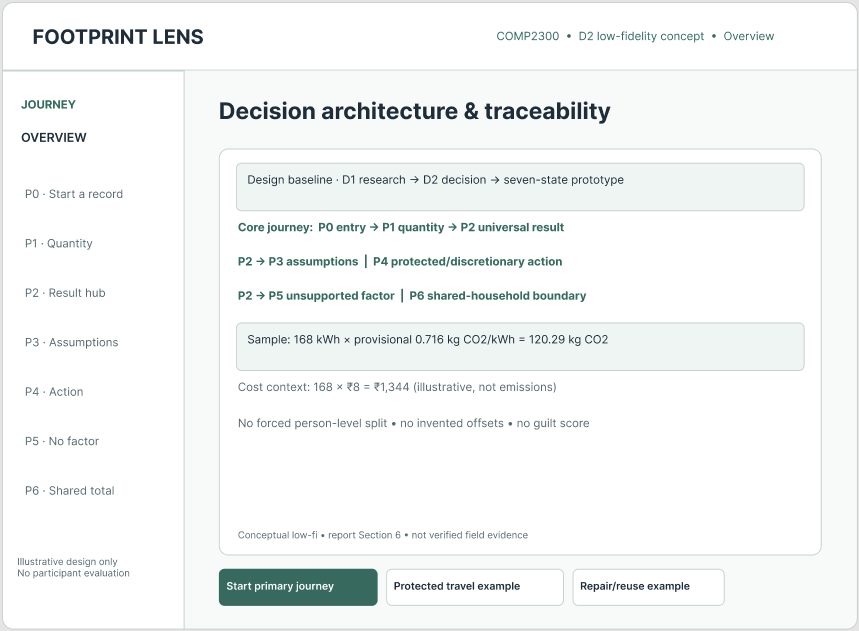
\includegraphics[width=0.60\textwidth,keepaspectratio]
{evidence/figma/overview.png}}

\caption{Figma overview: the P0--P2 core journey and optional P3--P6 routes. This is a navigation index, not a technical architecture.}
\label{fig:real-overview}
\end{figure}

% Core journey: entry
\begin{figure}[!htbp]
\centering
\figmarow
{P0 | Activity and scope}{4-12}{p0}
{P1 | Quantity and category-owned unit}{4-32}{p1}
\caption{Standard entry journey (US01a, US05a): scope and quantity are shown as fixed, low-fidelity examples.}
\label{fig:real-core}
\end{figure}

% Core journey: validation and result
\begin{figure}[!htbp]
\centering
\figmarow
{P1-E | Recoverable error}{4-42}{p1_e}
{P2 | Contextual result}{4-52}{p2}
\caption{Core journey continued: preserved input after validation and the illustrative 120.29 kg CO$_2$ result with separate rupee context.}
\label{fig:real-core-result}
\end{figure}

% Assumptions
\begin{figure}[!htbp]
\centering
\figmarow
{P3 | Assumption provenance}{4-72}{p3}
{P3-E | User-adjusted scenario}{4-82}{p3_e}
\caption{Assumption audit (US02a--b): a simulated factor change to 0.650 kg CO$_2$/kWh produces 109.20 kg CO$_2$, using frame switching rather than live calculation.}
\label{fig:real-provenance}
\end{figure}

% Protected journey: setup
\begin{figure}[!htbp]
\centering
\figmarow
{P0-B | Protected setup}{4-22}{p0_b}
{P1-T | Protected travel quantity}{5-2}{p1_t}
\caption{Protected-journey entry (US03a): a safety-critical trip is marked protected and recorded as 15 passenger-km.}
\label{fig:real-protected}
\end{figure}

% Protected journey: outcome
\begin{figure}[!htbp]
\centering
\figmarow
{P2-T | Travel result boundary}{5-22}{p2_t}
{P4-P | No unsafe substitution}{4-102}{p4_p}
\caption{Protected-journey outcome (US03a--b): unavailable factor disclosure and no unsafe substitution advice or penalty.}
\label{fig:real-protected-result}
\end{figure}

% Unsupported factor: entry
\begin{figure}[!htbp]
\centering
\figmarow
{P1-R | Repair / reuse input}{5-12}{p1_r}
{P2-U | Explicit unavailable result}{4-62}{p2_u}
\caption{Unsupported-category entry (US04a): repair/reuse remains descriptive when a defensible emissions factor is unavailable.}
\label{fig:real-unknown}
\end{figure}

% Unsupported factor: recovery
\begin{figure}[!htbp]
\centering
\figmarow
{P3-U | Missing-factor provenance}{5-32}{p3_u}
{P5 | Descriptive record}{4-112}{p5}
\caption{Unsupported-category recovery (US04b): inspect missing evidence without inventing offsets or treating unknown impact as zero.}
\label{fig:real-unknown-recovery}
\end{figure}

% Household privacy
\begin{figure}[!htbp]
\centering
\figmarow
{P6 | Communal by default}{4-122}{p6}
{P6-O | Explicit own-room consent}{4-132}{p6_o}
\caption{Household boundary (US07a--c): communal 168 kWh is not divided; a separate 40 kWh view uses independent input and consent.}
\label{fig:real-household}
\end{figure}

% Action decisions: proposed choice
\begin{figure}[!htbp]
\centering
\figmarow
{P4 | Optional action}{4-92}{p4}
{P4-C | Tentative choice}{5-42}{p4_c}
\caption{Non-punitive action decision (E3): the user can explore and provisionally choose a feasible suggestion.}
\label{fig:real-actions}
\end{figure}

% Action decisions: alternatives
\begin{figure}[!htbp]
\centering
\figmarow
{P4-D | Deferred}{5-52}{p4_d}
{P4-N | Not feasible}{5-62}{p4_n}
\caption{Action decisions continued: deferring or declining a suggestion produces no penalty or fabricated behavioural change.}
\label{fig:real-actions-alternatives}
\end{figure}

\endgroup
\FloatBarrier

\subsection{State-level behaviour and evidence map}
\begin{table}[ht]
\centering\small
\caption{State contract aligned to the linked Figma model and proposed implementation.}
\label{tab:state-contract}
\footnotesize\setlength{\tabcolsep}{4pt}
\renewcommand{\arraystretch}{1.3}
\rowcolors{2}{white}{RowGray!70}
\newcommand{\ids}[2]{#1\newline{\scriptsize\color{Slate}#2}}
\newcommand{\hdr}[1]{{\sffamily\bfseries\footnotesize\color{Navy}#1}}
\begin{tabularx}{\textwidth}{@{}>{\raggedright\arraybackslash\sffamily\bfseries\color{Teal}}p{1.0cm}
  >{\raggedright\arraybackslash\bfseries\color{Navy}}p{2.5cm}
  >{\raggedright\arraybackslash}X
  >{\raggedright\arraybackslash}p{2.9cm}@{}}
\toprule
\rowcolor{white}
\multicolumn{1}{@{}p{1.0cm}}{\hdr{State}}&
\multicolumn{1}{p{2.5cm}}{\hdr{Role}}&
\multicolumn{1}{>{\raggedright\arraybackslash}X}{\hdr{Required behaviour / return path}}&
\multicolumn{1}{p{2.9cm}@{}}{\hdr{Epic / child IDs}}\\
\midrule
P0&Entry and scope&Keep language, activity, communal/personal scope and protected flag visible.&\ids{E3, E5, E7}{US03a, US05b}\\
P1&Quantity and presets&Category owns unit; blank/negative/out-of-range rejected without erasing entries.&\ids{E1, E5}{US01a, US05a}\\
P2&Universal result&Every category reaches P2; unsupported factor is \emph{unavailable}, never zero.&\ids{E1, E2, E6}{US01b, US06a}\\
P3&Assumption audit&Source, year, geography, unit and formula stay visible during user edits.&\ids{E2, E9}{US02a--c}\\
P4&Feasible action&Protected path disables action choices without penalty; ordinary path offers decline/defer.&\ids{E3}{US03a--b}\\
P5&Descriptive recovery&No invented CO$_2$ credit for repair, reuse, waste or unknown-factor activities.&\ids{E4, E14}{US04a--b}\\
P6&Communal boundary&Household total never auto-divided; optional own-room attribution needs consent and independent data.&\ids{E7, E13}{US07a--c}\\
\bottomrule
\end{tabularx}
\end{table}

\begin{insightbox}{What the screenshots evidence -- and what they do not}
The linked screenshots document seven distinct decision responsibilities, recoverable and protected branches, factor transparency and a consent boundary. Their \textbf{breadth of conceptual behaviour} supports the D2 requirement to do more than log and display. They \textbf{do not} prove real data editing, networking, storage, Hindi localisation or success in participant testing; those require implementation and evaluation.
\end{insightbox}

\Needspace{18\baselineskip}\subsection{Proposed system architecture (D3 handover)}
\begin{figure}[H]
\centering
\resizebox{0.93\textwidth}{!}{%
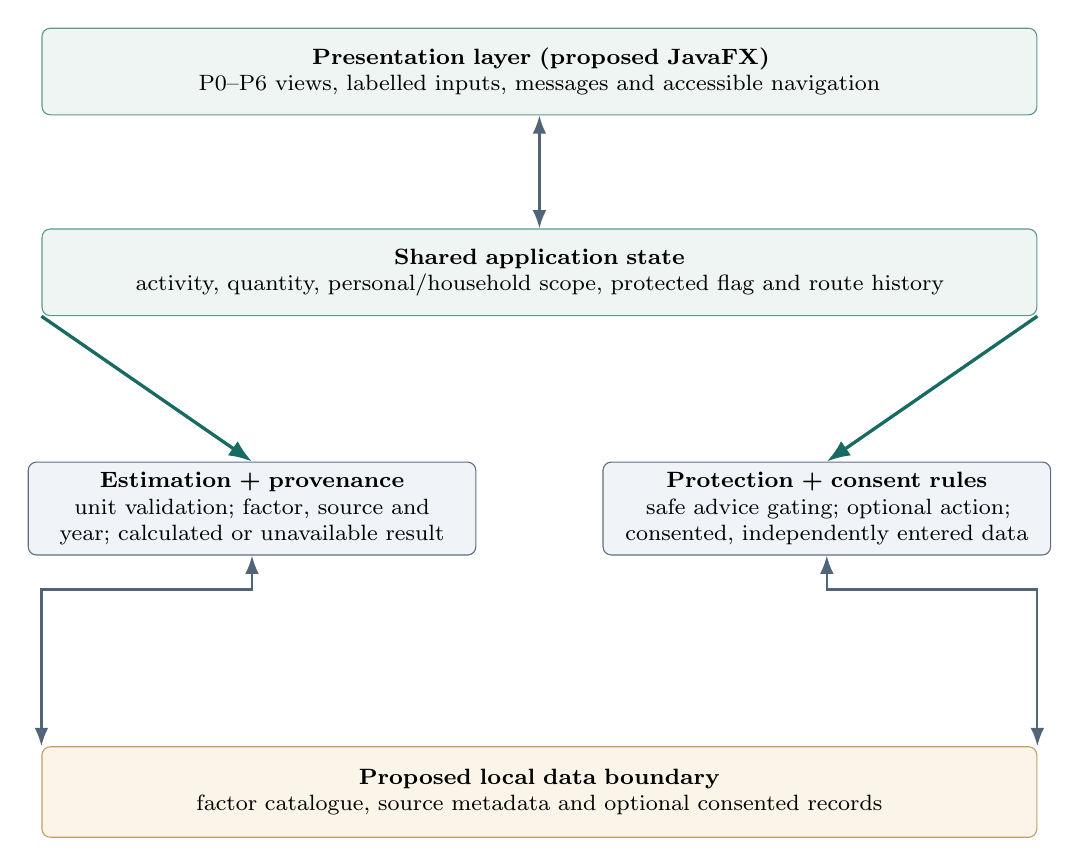
\begin{tikzpicture}[
  node distance=1cm,
  box/.style={draw=Teal!70,rounded corners=3pt,fill=TealPale,align=center,text width=12.4cm,minimum height=1.1cm,font=\footnotesize},
  service/.style={draw=Navy!70,rounded corners=3pt,fill=IndigoPale,align=center,text width=5.45cm,minimum height=1.18cm,font=\footnotesize},
  store/.style={draw=Amber!65,rounded corners=3pt,fill=AmberPale,align=center,text width=12.4cm,minimum height=1.15cm,font=\footnotesize},
  a/.style={-Latex,very thick,draw=Teal},
  b/.style={Latex-Latex,thick,draw=Slate}
]
\node[box] (ui) at (0,0) {\textbf{Presentation layer (proposed JavaFX)}\\ P0--P6 views, labelled inputs, messages and accessible navigation};
\node[box] (state) at (0,-2.55) {\textbf{Shared application state}\\ activity, quantity, personal/household scope, protected flag and route history};
\node[service] (calc) at (-3.65,-5.55) {\textbf{Estimation + provenance}\\ unit validation; factor, source and year; calculated or unavailable result};
\node[service] (choice) at (3.65,-5.55) {\textbf{Protection + consent rules}\\ safe advice gating; optional action; consented, independently entered data};
\node[store] (data) at (0,-9.15) {\textbf{Proposed local data boundary}\\ factor catalogue, source metadata and optional consented records};
\draw[b] (ui.south)--(state.north);
\draw[a] (state.south west) -- (calc.north);
\draw[a] (state.south east) -- (choice.north);
\draw[b] (calc.south)--++(0,-0.43)-|(data.north west);
\draw[b] (choice.south)--++(0,-0.43)-|(data.north east);
\end{tikzpicture}%
}
\caption{\textbf{Proposed high-level architecture, not an implementation diagram.} P0--P6 share explicit activity and constraint state, while separate deterministic services handle quantitative provenance and action/consent rules. Detailed UML, class responsibilities and deployment decisions belong to D3.}
\label{fig:architecture-image}
\end{figure}

\begin{keybox}
\textbf{Feasibility rationale.} Every proposed branch can be realised using JavaFX controls, deterministic validation and rule checks, and a small local catalogue of units/factors with source metadata. No speculative machine learning, live bank integration or cloud inference is necessary. \textbf{Detailed UML and technical design are reserved for D3}; this diagram is a conceptual bridge supporting D2 feasibility.
\end{keybox}

\begin{chapterfocus}{Accessibility is an acceptance concern, not a colour claim}
Controls need visible keyboard focus, readable labels, non-colour status text and appropriate announcements. The Figma frames communicate the intended hierarchy; full keyboard, screen-reader and Plain Hindi validation remain separate evaluation tasks.
\end{chapterfocus}

\subsection{Accessibility, Technical Feasibility and Verification}
The prototype specification includes accessibility requirements that should be verified during implementation and evaluation:
\begin{itemize}[leftmargin=*]
  \item \textbf{Keyboard operability:} All primary controls should be reachable in a logical tab order, expose a visible focus state, and support keyboard form submission.
  \item \textbf{Assistive-technology support:} Validation errors and dynamic status changes should be programmatically associated with their controls and announced to screen readers; route changes should move focus predictably.
  \item \textbf{Visual clarity:} Information should not rely on colour alone; text contrast, scalable layout and narrow-viewport reflow should be checked against the relevant accessibility criteria.
\end{itemize}
The project artefacts include eight pure-logic unit tests (\code{prototype-logic.test.mjs}) covering unit compatibility, calculations, protected states and boundaries, plus a structural contract check (\code{prototype-structure-check.py}) for selected IDs, panels and handlers. These checks support logic and structure verification; they do not establish WCAG conformance or successful screen-reader use. Retain the actual test output with the submission.

\Needspace{7\baselineskip}
\section{User Evaluation Protocol for D3/D7}

To support the required D2 evaluation plan and later D3/D7 testing, we specify a controlled, task-based study. This is a proposed protocol, not results:

\subsection{Participant Selection and Ethics}
The proposed study targets up to $N=6$ participants recruited from \emph{other} COMP2300 project groups, subject to availability, consent, and the module restrictions \cite{modulebrief}. Recruitment should seek variation across student/shared-housing, working-professional and household-management contexts; this convenience sample will not represent the wider Indian population. To ensure ethical integrity, no sensitive personal energy bills, financial records, or location histories will be collected; all tasks will utilize standardized synthetic scenarios. Participants will complete an informed consent form and debriefing.

\subsection{Structured Task Scenarios}
\begin{enumerate}[label=\textbf{Task \arabic*:},leftmargin=*]
  \item \textbf{Standard Activity Logging and Provenance Check (E1, E2):} Participant receives the fixed 168 kWh household scenario in the Figma click-through (or a 150 kWh personal synthetic bill in the separate functional simulator/future implementation). They navigate P0--P3 and identify the conversion factor, its unverified year status and scope; quantitative entry is assessed only in a build that actually accepts it.
  \item \textbf{Constraint Protection (E3):} Participant is asked to review a late-night safety-cab commute (15 passenger-km) undertaken for personal safety. They must mark the routine as protected, proceed to P4, and explain why action buttons are disabled.
  \item \textbf{Descriptive Logging for Unsupported Category (E4):} Participant follows the Figma repair/reuse descriptive route for 1 item (or logs 3 kg delivery packaging in a functional implementation), opens P5 and verifies that no numerical credit is fabricated.
  \item \textbf{Shared Boundary Comprehension (E1, E7):} Participant inspects the Figma 168 kWh household electricity total (or a 500 kWh synthetic bill in a functional implementation), navigates to P6, and answers an explain-back comprehension question regarding whether this total can be attributed to them individually.
\end{enumerate}

\subsection{Moderation and question protocol}
Each participant receives the same synthetic task data and a neutral briefing. The moderator records actions and errors without prompting an answer; afterwards the participant is asked: \emph{``What does this number mean, and how confident are you in it?''}, \emph{``Would a shared electricity bill tell you your personal footprint? Why?''}, and \emph{``Was any suggestion inappropriate for the stated safety constraint?''} These are comprehension and perceived-pressure probes, not questions about the participant's actual health, finances, commuting history or identity. Sessions take place in a controlled quiet room with participants from another COMP2300 group, as required by the module brief \cite{modulebrief}.

\subsection{Evaluation Metrics}
\begin{itemize}[leftmargin=*]
  \item \textbf{Effectiveness:} Task Completion Rate (binary success/failure per task); Critical Error Rate (submitting invalid data without recovery).
  \item \textbf{Efficiency:} Time on Task (target: $\le 60$ seconds for Task 1); Total interaction step count.
  \item \textbf{Cognitive Comprehension:} Post-task explain-back probes verifying whether participants understood that illustrative numbers are not verified emissions.
  \item \textbf{Usability and Satisfaction:} Single Ease Question (SEQ, 1--7 scale) after each task; System Usability Scale (SUS) questionnaire administered post-session, with a interpretive benchmark of $\ge 75/100$, not a guaranteed outcome or pass criterion.
\end{itemize}

For consistency, task completion should be recorded as successful only when the participant reaches the intended state and correctly explains the key boundary being tested. Time-on-task should be measured from the first task instruction to completion; assistance and critical errors should be logged separately. Results should be reported descriptively (counts, ranges and representative observations) because a small convenience sample does not support broad statistical generalisation.

\Needspace{7\baselineskip}
\section{Three-Week Design Progression and Work Products}

The report is organised around three substantial design work packages. This timeline is an artefact-based reconstruction of the progression represented by the D1 baseline, concept alternatives, story register, flowcharts and prototype specification. It should be checked against the team's actual meeting notes and any dated design artefacts before submission; it is not a substitute for records of work actually undertaken.

\begin{table}[ht]
\centering
\small
\caption{Three-week progression of the conceptual design work}
\label{tab:three-week}
\begin{tabularx}{\textwidth}{@{}p{1.5cm}p{3.2cm}Xp{3.2cm}@{}}
\toprule
\textbf{Period} & \textbf{Design focus} & \textbf{Work products represented in this report} & \textbf{Exit condition}\\
\midrule
\textbf{Week 1} & Problem framing and requirements translation & Revisited D1 personas, scenarios, semantic/latent themes and epics; articulated the JTBD; converted research implications into five design principles and explicit constraints. & Each principle is traceable to a D1 driver and a proposed interaction control.\\
\rowcolor{brandlight}
\textbf{Week 2} & Divergent exploration and concept convergence & Consolidated eight response families; developed three distinct interaction paradigms; compared their stakeholder fit, feasibility, transparency and socio-technical risks using weighted MCDM. & One concept selected with documented trade-offs and rejected alternatives.\\
\textbf{Week 3} & Specification, interaction architecture and verification planning & Decomposed the selected concept into P0--P6; specified prioritised stories and BDD acceptance criteria; refined flowcharts, low-fidelity screens, architecture direction, risks and a formative evaluation protocol. & A traceable conceptual specification ready for prototype evaluation and subsequent implementation planning.\\
\bottomrule
\end{tabularx}
\end{table}

The progression shows increasing design resolution: from \emph{why} the system is needed, to \emph{which} interaction model best addresses the problem, to \emph{how} the selected model should behave and be evaluated. The work products are linked rather than independent: the design principles constrain the concept selection; the selected concept determines the P0--P6 flow; the flow is decomposed into user stories; and the acceptance criteria inform the evaluation tasks and later test design.

\subsection{Traceability and Change Control}
A change to an epic, persona constraint or interaction state should be propagated through the story register, flowchart, wireframe and evaluation task that depend on it. For the next iteration, the team should maintain a lightweight change record with: (1) the source requirement or D1 finding, (2) the affected story/state, (3) the design change, (4) the rationale, and (5) the verification case. This reduces requirements drift and makes review feedback auditable.

\Needspace{7\baselineskip}
\section{D2 Collaboration, Process Reflection and D3 Handover}

\subsection{D2 Collaboration and Team Responsibilities}

The D2 deliverables were developed primarily through the collaborative work of Arnav Mishra and Keshav Singhal, who undertook the principal research-to-design, documentation and technical development responsibilities. Their contributions covered complementary areas of the project, with regular discussion and cross-review helping maintain consistency across the report, prototype and supporting evidence.
\begin{itemize}[leftmargin=*]
  \item \textbf{Arnav Mishra (Research, Design and Documentation):} Led the development and refinement of the D2 report, connecting D1 research findings to design principles, user stories and acceptance criteria. Also contributed to prototyping, design ideation, flowcharts, meeting minutes and quality assurance.

  \item \textbf{Keshav Singhal (Engineering and Technical Development):} Led the calculation logic, test design and technical feasibility work. Also contributed to MoSCoW prioritisation, architecture planning, prototype verification and reviewing the technical specifications.
\end{itemize}
Both worked closely on design discussions, reviewing deliverables and resolving inconsistencies to maintain alignment between the report, prototype and technical specifications. Supporting evidence includes report drafts, diagrams, test files, meeting records and Figma frames. GitLab workflows, issue tracking and merge-request reviews remain proposed practices for D3 rather than completed D2 activities.

\subsection{D3 Handover: Proposed GitLab Workflow}
\begin{insightbox}{Starting in D3 | GitLab is a plan, not D2 evidence}
Beginning with D3, the team \textbf{aims to maintain a shared GitLab repository} for the Java/JavaFX implementation. The proposed workflow is to track small stories and bugs as issues, use feature branches and merge requests for reviewed changes, link tests to acceptance criteria, and document key decisions. These practices are future intentions; this D2 report makes \textbf{no claim} that the workflow, commits or review history already exists.
\end{insightbox}

\subsection{Critical Process Reflection}
The transition from D1 to D2 underscored the vital distinction between user intentions and structural feasibility. The alternative concepts and working notes explore bill scanning, shared displays and asynchronous cards. These options introduce distinct foreseeable risks: parsing and privacy for scanning, consent and shared-display exposure for household boards, and weaker immediate provenance for weekly cards. Concept A was selected as a bounded way to test transparent estimates and feasible advice without depending on automated data ingestion or speculative machine learning. The team's next review must also consider the cost of manual entry and whether the extra assumption screen actually improves comprehension.

%\Needspace{7\baselineskip}

\Needspace{8\baselineskip}
\section{Design Evidence, Verification and Limitations}
\label{sec:design-evidence}

\subsection{Design and Collaboration Evidence}

The conceptual development of \textbf{Footprint Lens} is documented through the Deliverable 1 research baseline, three alternative design concepts, prioritised user stories, annotated ideation sketches, interaction diagrams, and the linked Figma low-fidelity prototype.

Appendix~\ref{app:ideation} presents three annotated design sheets illustrating divergent problem responses, comparison of competing concepts, and refinement of the selected \textit{Contextual Choice Coach}. Together, these artefacts make the progression from initial design possibilities to the chosen interaction model more transparent. The sheets include handwritten annotations and, where indicated, printed visual references. They are presented as design-review evidence rather than proof of an independently observed or dated historical workshop.

The team's meeting minutes provide supporting records of discussions, design decisions, responsibilities, and project progression where those activities are documented. Peer assessments and individual reflections provide complementary accounts of collaboration and contribution through the module's separate submission arrangements. These records support process accountability without substituting for evidence of the prototype's usability.

\subsection{Prototype Verification}

The low-fidelity prototype consists of \textbf{21 linked Figma frames}, organised around the seven principal states (P0--P6) and their relevant interaction variants.

The team's internal walkthrough confirms the basic clickable navigation through representative scenarios, including activity entry, quantity validation, assumption inspection, protected routines, unavailable estimates, and voluntary household attribution.

The report also describes a separate browser-based logic simulator and supporting deterministic checks. These are distinguished from the Figma click-through: the former exercise selected calculation and state rules, while the latter communicates the intended interaction through predefined screen states.

\begin{insightbox}{Evidence of the proposed interaction design}
\textbf{Demonstrated:} A linked conceptual journey, representative decision branches, validation feedback, transparent assumption displays, and explicit safety and privacy boundaries.

\textbf{Not yet demonstrated:} Production-ready data processing, live calculation within Figma, persistent user records, complete localisation, or successful usability and accessibility testing with representative participants.

This distinction preserves the intended low fidelity of D2 while making the scope of the available evidence explicit.
\end{insightbox}

\subsection{Limitations and Future Verification}

The prototype is an exploratory design artefact rather than a completed application. Its fixed-state interactions demonstrate proposed behaviour but do not establish that the experience is equally understandable, accessible, or effective for all six D1 personas.

Quantitative examples retain their documented evidence boundaries. The illustrative electricity factor of $0.716\,\mathrm{kg\,CO_2/kWh}$ remains provisional unless supported by an authoritative, dated source. The assumed electricity tariff of Rs.~8/kWh provides cost context rather than a universal tariff. Repair and reuse activities are represented without fabricated avoided-emissions credits.

The formative evaluation described in Section~7 will investigate task comprehension, accessibility, perceived pressure, and the suitability of the design for users with different practical constraints. Detailed technical architecture, development infrastructure, and implementation verification are reserved for subsequent deliverables.

The resulting D2 artefacts therefore provide a traceable and technically plausible foundation for evaluation and implementation, while distinguishing design intentions from established findings.

\section{Conclusion and D3 Handover}
Deliverable 2 translates the D1 research baseline into three distinct conceptual alternatives, selects Concept A through weighted decision analysis, and develops a traceable backlog and low-fidelity interaction model. These artefacts provide a foundation for formative evaluation and subsequent implementation in D3. The prototype logic and document structure are supported by automated checks among the supplied project files; however, these do not replace moderated user evaluation, accessibility testing with assistive technologies or verification of the final design against user needs. D3 will build on this specification through detailed technical design, implementation and further testing, while addressing the limitations identified in Section~10.
\vspace{0.45cm}
\noindent{\color{Teal}\rule{\linewidth}{0.8pt}}
\begingroup
\setlength{\parskip}{0.15em}
\begin{thebibliography}{12}
\small
\setlength{\itemsep}{-0.16em}
\setlength{\parsep}{0pt}
\bibitem{modulebrief} University of Southampton, COMP2300 Module Team. 2026. \emph{COMP2300 Software Design and Development Project: Coursework Specification 2026/27}. Internal module assessment brief; D2 section and marking rubric.
\bibitem{d1report} A. Mishra, K. Singhal and H. Makkar. 2026. \emph{Carbon Footprint Awareness and Reduction Tool: India-Centric Challenge}. COMP2300 Deliverable 1: Problem-Space Research and Product Definition, submitted 23 October 2026. Internal team report.
\bibitem{earthhero} Earth Hero. 2026. \emph{Climate Action App}. \url{https://www.earthhero.org/app/}. Product description accessed 17 November 2026; coverage may change.
\bibitem{gikizero} Giki Zero / AEP Energy. 2026. \emph{Giki Zero personal carbon-footprint tool}. \url{https://www.aepenergy.com/residential/renewable-energy/giki-zero/}. Product description accessed 17 November 2026.

\bibitem{hoffmann2024} S. Hoffmann, W. Lasarov, H. Reimers and M. Trabandt. 2024. Carbon footprint tracking apps. Does feedback help reduce carbon emissions? \emph{Journal of Cleaner Production} 434, 139981. DOI: \href{https://doi.org/10.1016/j.jclepro.2023.139981}{10.1016/j.jclepro.2023.139981}.
\bibitem{lasarov2024} W. Lasarov, S. Hoffmann, R. Mai and J. Schleich. 2024. Carbon footprint tracking apps: the spillover effects of feedback and goal-activating appeals. \emph{Ecological Economics} 226, 108354. DOI: \href{https://doi.org/10.1016/j.ecolecon.2024.108354}{10.1016/j.ecolecon.2024.108354}.
\bibitem{brynjarsdottir2012} H. Brynjarsdottir, M. Hakansson, J. Pierce, E. Baumer, C. DiSalvo and P. Sengers. 2012. Sustainably unpersuaded: How persuasion narrows our vision of sustainability. In \emph{Proc. ACM CHI '12}. ACM, 947--956. DOI: \href{https://doi.org/10.1145/2207676.2208539}{10.1145/2207676.2208539}.
\bibitem{lee2021} J. Lee, O. Taherzadeh and K. Kanemoto. 2021. The scale and drivers of carbon footprints in households, cities and regions across India. \emph{Global Environmental Change} 66, 102205. DOI: \href{https://doi.org/10.1016/j.gloenvcha.2020.102205}{10.1016/j.gloenvcha.2020.102205}.
\bibitem{mohanty2023} V. Mohanty, A. Filipowicz, N. Bravo, S. Carter and D. A. Shamma. 2023. Save a tree or 6 kg of CO2? In \emph{Proc. ACM CHI '23}. ACM. DOI: \href{https://doi.org/10.1145/3544548.3580675}{10.1145/3544548.3580675}.
\bibitem{shi2021} S. Shi and J. Yin. 2021. Global research on carbon footprint: A scientometric review. \emph{Environmental Impact Assessment Review} 89, 106571. DOI: \href{https://doi.org/10.1016/j.eiar.2021.106571}{10.1016/j.eiar.2021.106571}.
\end{thebibliography}
\endgroup


\clearpage
\appendix
\renewcommand{\thefigure}{A.\arabic{figure}}
\setcounter{figure}{0}
\section{Annotated Ideation and Concept Development Sketches}\label{app:ideation}

These three annotated sketches supplement the concept arguments in Sections~2--4. Supplied on 19 November 2026, they illustrate design-review reasoning; the original session date and individual contributions require team confirmation. Printed visual references are identified where present. The final concept flow and Figma frames supersede early sketch arrangements.

\subsection{Divergent problem responses}
\begin{figure}[H]
\centering
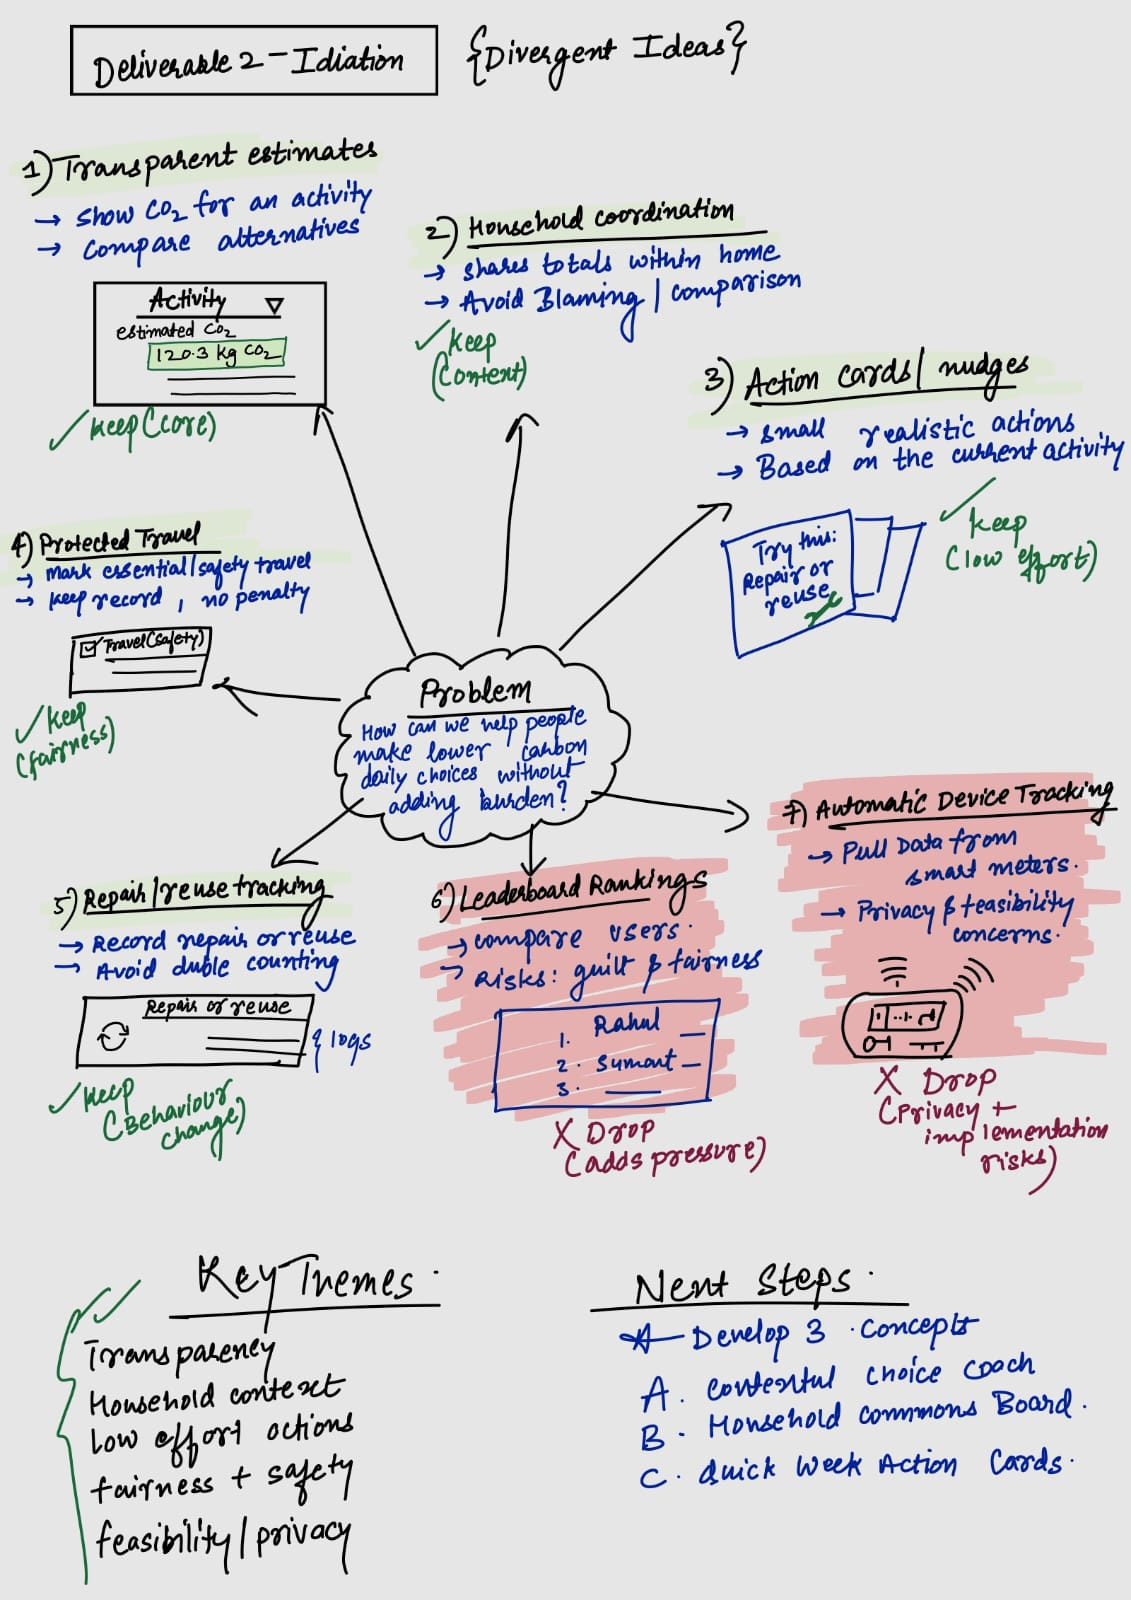
\includegraphics[width=0.84\textwidth,height=15.7cm,keepaspectratio]{evidence/sketches/divergent.jpg}
\caption{Annotated divergent-ideas sheet. Seven visible strands explore estimates, household coordination, action cards, protected travel, repair/reuse, leaderboards and automation, with stated keep/drop reasons. This is a design-review sketch, not a dated user study.}
\label{fig:sketch_divergent}
\end{figure}
\clearpage

\subsection{Three competing concept sketches}
\begin{figure}[H]
\centering
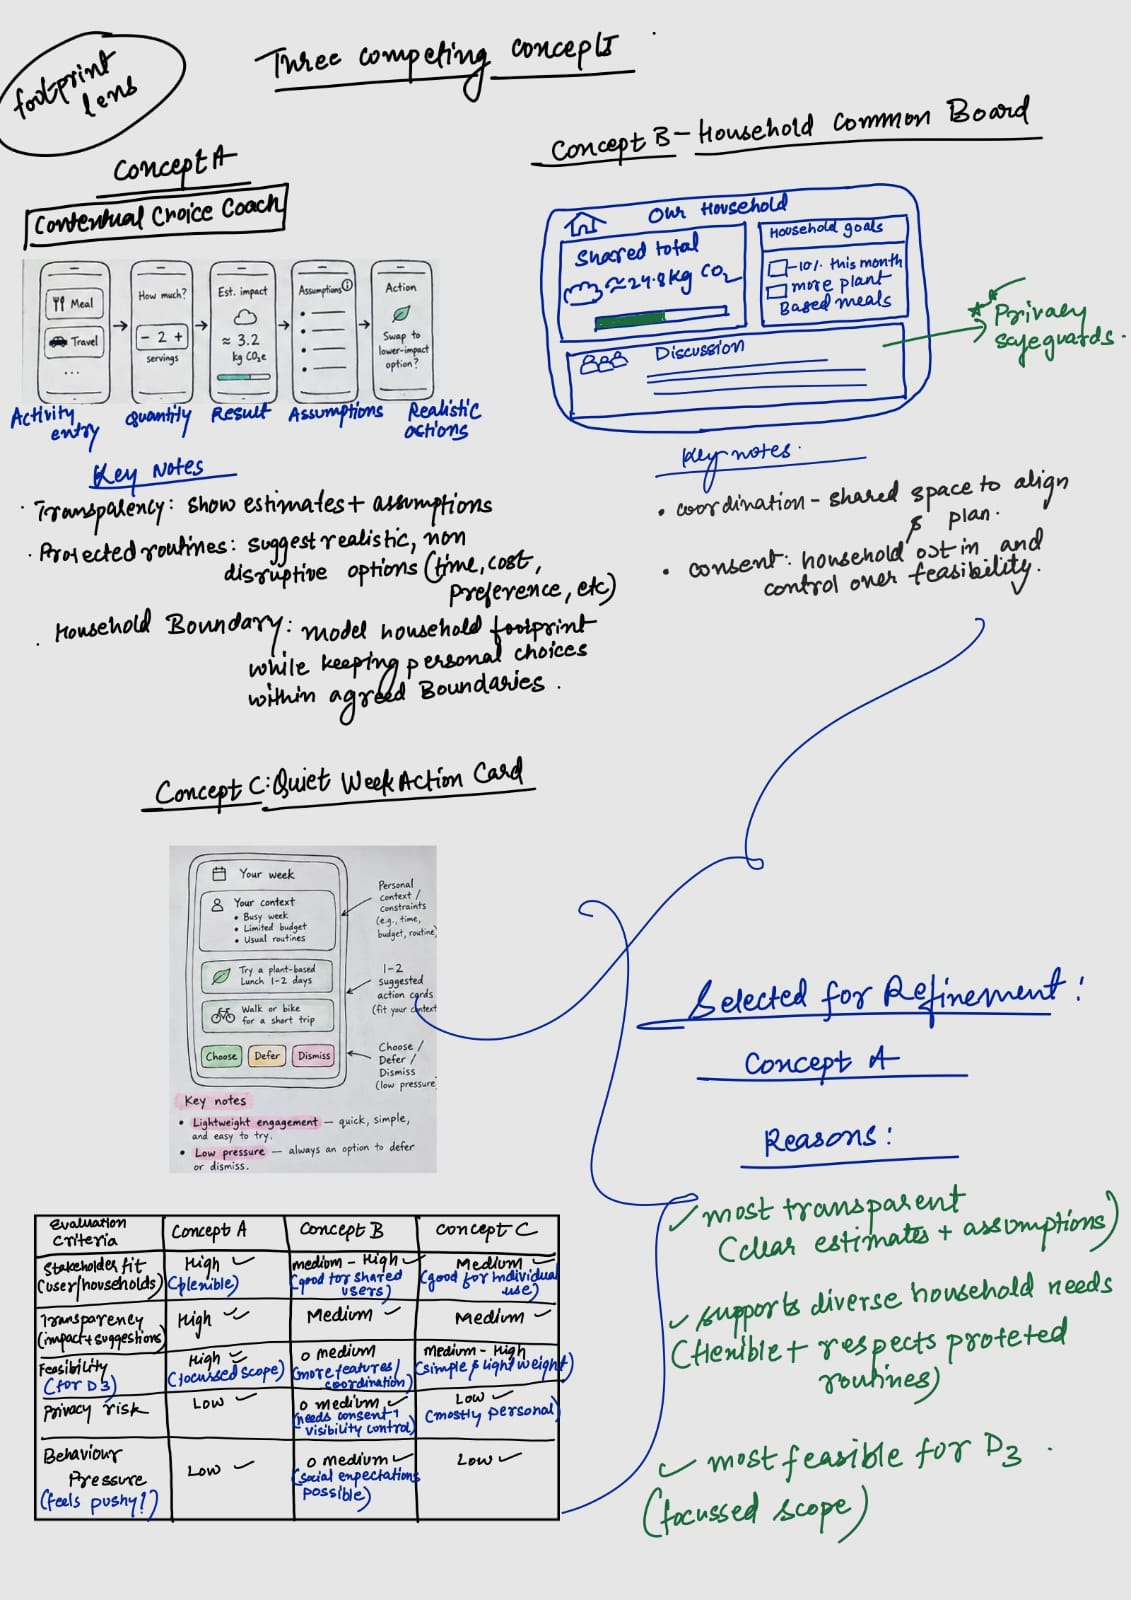
\includegraphics[width=0.89\textwidth,height=21.0cm,keepaspectratio]{evidence/sketches/concepts.jpg}
\caption{Concept A (Contextual Choice Coach), B (Household Commons Board) and C (Quiet-Week Action Cards), with a handwritten comparison of stakeholder fit, transparency, feasibility and social pressure. Concept C includes a printed visual reference with handwritten annotations; the comparison is a design rationale rather than measured user preferences.}
\label{fig:sketch_concepts}
\end{figure}
\clearpage

\subsection{Concept A refinement and accepted trade-offs}
\begin{figure}[H]
\centering
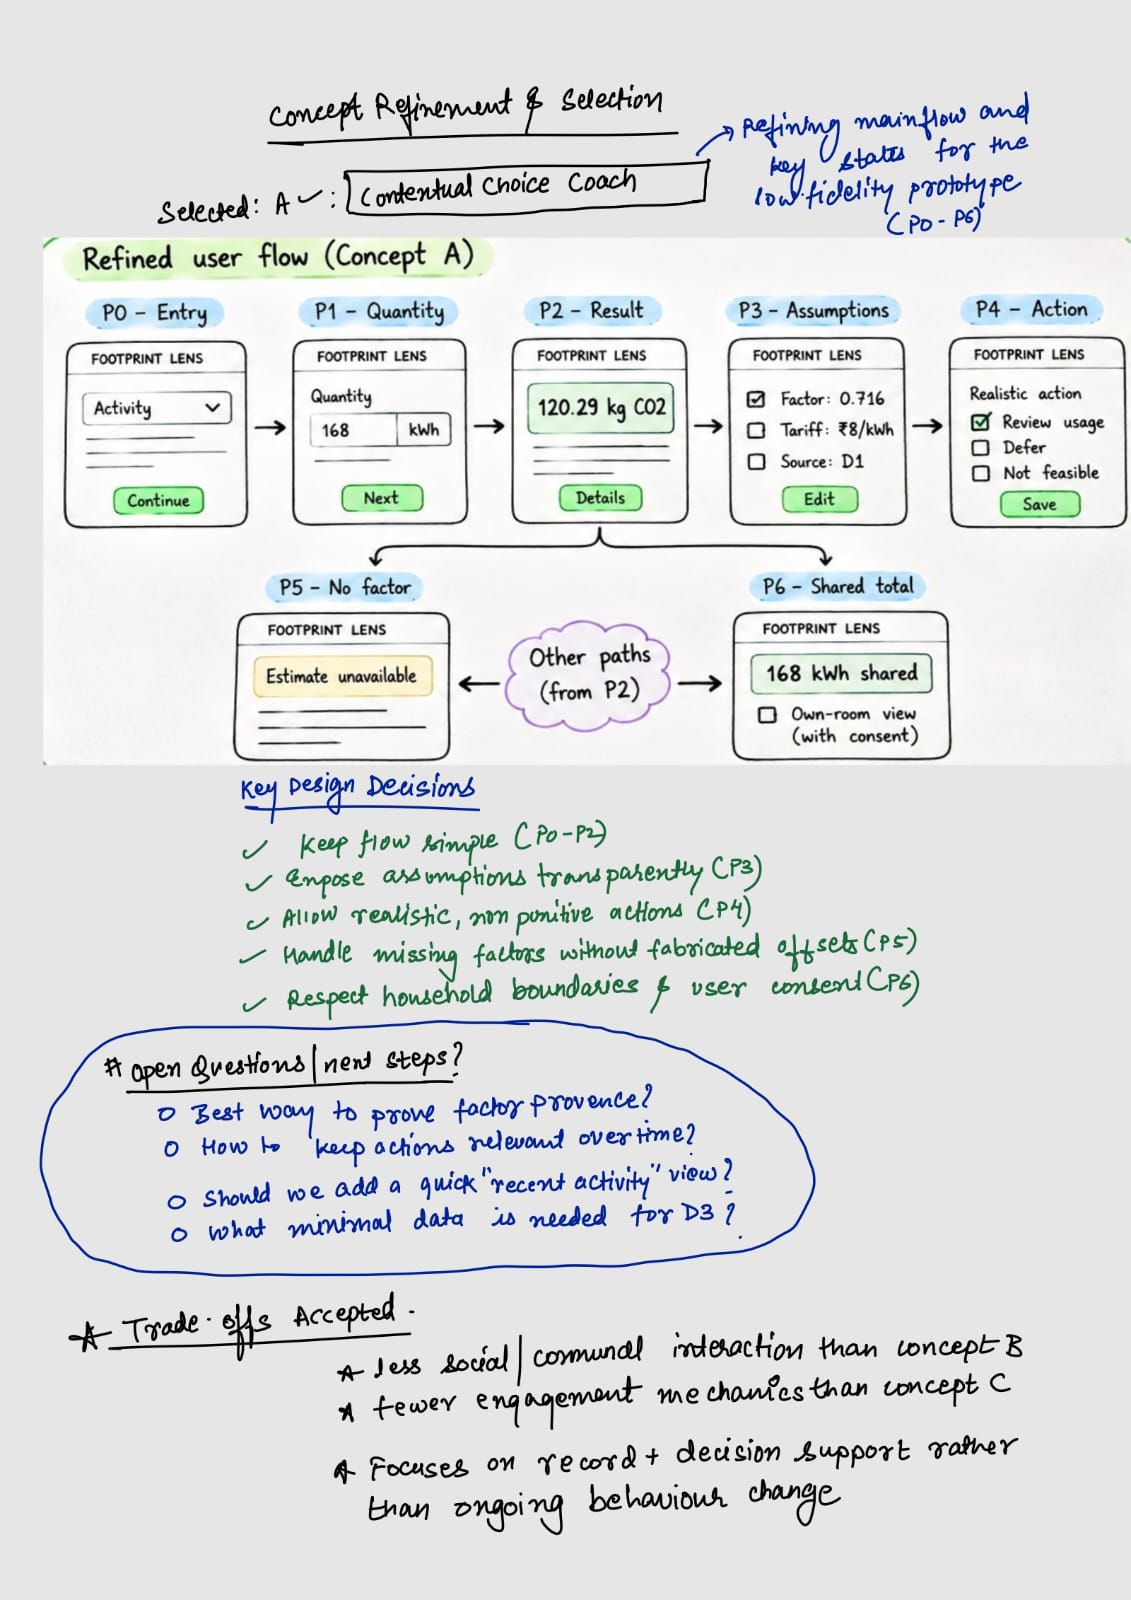
\includegraphics[width=0.89\textwidth,height=20.8cm,keepaspectratio]{evidence/sketches/refinement.jpg}
\caption{Annotated refinement sheet for the selected Contextual Choice Coach, including design principles, open questions and accepted trade-offs. The pasted flow illustration sketches P3/P4 sequentially; the revised interaction contract branches P3--P6 from P2 as shown in the final state diagram and Figma prototype.}
\label{fig:sketch_refinement}
\end{figure}

\end{document}